% Options for packages loaded elsewhere
\PassOptionsToPackage{unicode}{hyperref}
\PassOptionsToPackage{hyphens}{url}
\documentclass[
]{book}
\usepackage{xcolor}
\usepackage{amsmath,amssymb}
\setcounter{secnumdepth}{5}
\usepackage{iftex}
\ifPDFTeX
  \usepackage[T1]{fontenc}
  \usepackage[utf8]{inputenc}
  \usepackage{textcomp} % provide euro and other symbols
\else % if luatex or xetex
  \usepackage{unicode-math} % this also loads fontspec
  \defaultfontfeatures{Scale=MatchLowercase}
  \defaultfontfeatures[\rmfamily]{Ligatures=TeX,Scale=1}
\fi
\usepackage{lmodern}
\ifPDFTeX\else
  % xetex/luatex font selection
\fi
% Use upquote if available, for straight quotes in verbatim environments
\IfFileExists{upquote.sty}{\usepackage{upquote}}{}
\IfFileExists{microtype.sty}{% use microtype if available
  \usepackage[]{microtype}
  \UseMicrotypeSet[protrusion]{basicmath} % disable protrusion for tt fonts
}{}
\makeatletter
\@ifundefined{KOMAClassName}{% if non-KOMA class
  \IfFileExists{parskip.sty}{%
    \usepackage{parskip}
  }{% else
    \setlength{\parindent}{0pt}
    \setlength{\parskip}{6pt plus 2pt minus 1pt}}
}{% if KOMA class
  \KOMAoptions{parskip=half}}
\makeatother
\usepackage{color}
\usepackage{fancyvrb}
\newcommand{\VerbBar}{|}
\newcommand{\VERB}{\Verb[commandchars=\\\{\}]}
\DefineVerbatimEnvironment{Highlighting}{Verbatim}{commandchars=\\\{\}}
% Add ',fontsize=\small' for more characters per line
\usepackage{framed}
\definecolor{shadecolor}{RGB}{248,248,248}
\newenvironment{Shaded}{\begin{snugshade}}{\end{snugshade}}
\newcommand{\AlertTok}[1]{\textcolor[rgb]{0.94,0.16,0.16}{#1}}
\newcommand{\AnnotationTok}[1]{\textcolor[rgb]{0.56,0.35,0.01}{\textbf{\textit{#1}}}}
\newcommand{\AttributeTok}[1]{\textcolor[rgb]{0.13,0.29,0.53}{#1}}
\newcommand{\BaseNTok}[1]{\textcolor[rgb]{0.00,0.00,0.81}{#1}}
\newcommand{\BuiltInTok}[1]{#1}
\newcommand{\CharTok}[1]{\textcolor[rgb]{0.31,0.60,0.02}{#1}}
\newcommand{\CommentTok}[1]{\textcolor[rgb]{0.56,0.35,0.01}{\textit{#1}}}
\newcommand{\CommentVarTok}[1]{\textcolor[rgb]{0.56,0.35,0.01}{\textbf{\textit{#1}}}}
\newcommand{\ConstantTok}[1]{\textcolor[rgb]{0.56,0.35,0.01}{#1}}
\newcommand{\ControlFlowTok}[1]{\textcolor[rgb]{0.13,0.29,0.53}{\textbf{#1}}}
\newcommand{\DataTypeTok}[1]{\textcolor[rgb]{0.13,0.29,0.53}{#1}}
\newcommand{\DecValTok}[1]{\textcolor[rgb]{0.00,0.00,0.81}{#1}}
\newcommand{\DocumentationTok}[1]{\textcolor[rgb]{0.56,0.35,0.01}{\textbf{\textit{#1}}}}
\newcommand{\ErrorTok}[1]{\textcolor[rgb]{0.64,0.00,0.00}{\textbf{#1}}}
\newcommand{\ExtensionTok}[1]{#1}
\newcommand{\FloatTok}[1]{\textcolor[rgb]{0.00,0.00,0.81}{#1}}
\newcommand{\FunctionTok}[1]{\textcolor[rgb]{0.13,0.29,0.53}{\textbf{#1}}}
\newcommand{\ImportTok}[1]{#1}
\newcommand{\InformationTok}[1]{\textcolor[rgb]{0.56,0.35,0.01}{\textbf{\textit{#1}}}}
\newcommand{\KeywordTok}[1]{\textcolor[rgb]{0.13,0.29,0.53}{\textbf{#1}}}
\newcommand{\NormalTok}[1]{#1}
\newcommand{\OperatorTok}[1]{\textcolor[rgb]{0.81,0.36,0.00}{\textbf{#1}}}
\newcommand{\OtherTok}[1]{\textcolor[rgb]{0.56,0.35,0.01}{#1}}
\newcommand{\PreprocessorTok}[1]{\textcolor[rgb]{0.56,0.35,0.01}{\textit{#1}}}
\newcommand{\RegionMarkerTok}[1]{#1}
\newcommand{\SpecialCharTok}[1]{\textcolor[rgb]{0.81,0.36,0.00}{\textbf{#1}}}
\newcommand{\SpecialStringTok}[1]{\textcolor[rgb]{0.31,0.60,0.02}{#1}}
\newcommand{\StringTok}[1]{\textcolor[rgb]{0.31,0.60,0.02}{#1}}
\newcommand{\VariableTok}[1]{\textcolor[rgb]{0.00,0.00,0.00}{#1}}
\newcommand{\VerbatimStringTok}[1]{\textcolor[rgb]{0.31,0.60,0.02}{#1}}
\newcommand{\WarningTok}[1]{\textcolor[rgb]{0.56,0.35,0.01}{\textbf{\textit{#1}}}}
\usepackage{longtable,booktabs,array}
\usepackage{calc} % for calculating minipage widths
% Correct order of tables after \paragraph or \subparagraph
\usepackage{etoolbox}
\makeatletter
\patchcmd\longtable{\par}{\if@noskipsec\mbox{}\fi\par}{}{}
\makeatother
% Allow footnotes in longtable head/foot
\IfFileExists{footnotehyper.sty}{\usepackage{footnotehyper}}{\usepackage{footnote}}
\makesavenoteenv{longtable}
\usepackage{graphicx}
\makeatletter
\newsavebox\pandoc@box
\newcommand*\pandocbounded[1]{% scales image to fit in text height/width
  \sbox\pandoc@box{#1}%
  \Gscale@div\@tempa{\textheight}{\dimexpr\ht\pandoc@box+\dp\pandoc@box\relax}%
  \Gscale@div\@tempb{\linewidth}{\wd\pandoc@box}%
  \ifdim\@tempb\p@<\@tempa\p@\let\@tempa\@tempb\fi% select the smaller of both
  \ifdim\@tempa\p@<\p@\scalebox{\@tempa}{\usebox\pandoc@box}%
  \else\usebox{\pandoc@box}%
  \fi%
}
% Set default figure placement to htbp
\def\fps@figure{htbp}
\makeatother
\setlength{\emergencystretch}{3em} % prevent overfull lines
\providecommand{\tightlist}{%
  \setlength{\itemsep}{0pt}\setlength{\parskip}{0pt}}
\usepackage[]{natbib}
\bibliographystyle{plainnat}
\usepackage{booktabs}
\usepackage{bookmark}
\IfFileExists{xurl.sty}{\usepackage{xurl}}{} % add URL line breaks if available
\urlstyle{same}
\hypersetup{
  pdftitle={Week 11: Censored Models and Sample Selection},
  pdfauthor={Samuel Rowe adapted from Wooldridge (2011), Mitchell (2020), and UCLA OARC (2025)},
  hidelinks,
  pdfcreator={LaTeX via pandoc}}

\title{Week 11: Censored Models and Sample Selection}
\author{Samuel Rowe adapted from Wooldridge (2011), Mitchell (2020), and UCLA OARC (2025)}
\date{2025-11-19}

\begin{document}
\maketitle

{
\setcounter{tocdepth}{1}
\tableofcontents
}
\begin{Shaded}
\begin{Highlighting}[]
\NormalTok{bookdown}\SpecialCharTok{::}\FunctionTok{render\_book}\NormalTok{()}
\end{Highlighting}
\end{Shaded}

\chapter*{Overview}\label{overview}
\addcontentsline{toc}{chapter}{Overview}

This week we will be covering:

\begin{enumerate}
\def\labelenumi{\arabic{enumi}.}
\tightlist
\item
  Censored Regression Models
\item
  Truncated Regression Models
\item
  Sample Selection
\item
  Subgroup Functions Part II
\end{enumerate}

\chapter{Censored Models}\label{censored-models}

\section{Censored Regression Model - Right-Censoring}\label{censored-regression-model---right-censoring}

\textbf{Lesson: We can use a Tobit estimator for right-censored model}

We need to summarize the dependent variable to see the right-censored value. We know that weekly earnings in the Current Population Survey are top-coded or right-censored at \$2884.61. This may bias our estimate, so we'll compare a OLS model and a Tobit model for right-censored data. Remember a Tobit estimator for a censored model is different from a corner solution.

\begin{Shaded}
\begin{Highlighting}[]
\KeywordTok{use} \StringTok{"/Users/Sam/Desktop/Econ 645/Data/CPS/jan2024.dta"}\NormalTok{, }\KeywordTok{clear}
\KeywordTok{sum}\NormalTok{ earnings }\KeywordTok{if}\NormalTok{ prerelg==1, }\KeywordTok{detail}
\KeywordTok{histogram}\NormalTok{ earnings }\KeywordTok{if}\NormalTok{ prerelg==1, }\FunctionTok{normal} \BaseNTok{title}\NormalTok{(Histogram }\KeywordTok{of}\NormalTok{ Weekly Earnings) }\BaseNTok{caption}\NormalTok{(}\StringTok{"Source: Current Population Survey"}\NormalTok{)}
\KeywordTok{graph} \KeywordTok{export} \StringTok{"/Users/Sam/Desktop/Econ 645/R Markdown/week9\_histogram\_earnings.png"}\NormalTok{, }\KeywordTok{replace}
\end{Highlighting}
\end{Shaded}

\begin{verbatim}
                  Weekly Earnings: pternwa
-------------------------------------------------------------
      Percentiles      Smallest
 1%           70              0
 5%          225              0
10%          360              0       Obs              10,666
25%          656              0       Sum of Wgt.      10,666

50%         1000                      Mean           1230.474
                        Largest       Std. Dev.      788.1457
75%         1680        2884.61
90%       2692.3        2884.61       Variance       621173.7
95%      2884.61        2884.61       Skewness       .7779644
99%      2884.61        2884.61       Kurtosis       2.648218

(bin=40, start=0, width=72.11525)

(file /Users/Sam/Desktop/Econ 645/R Markdown/week9_histogram_earnings.png written in PNG format)
\end{verbatim}

\begin{figure}
\centering
\pandocbounded{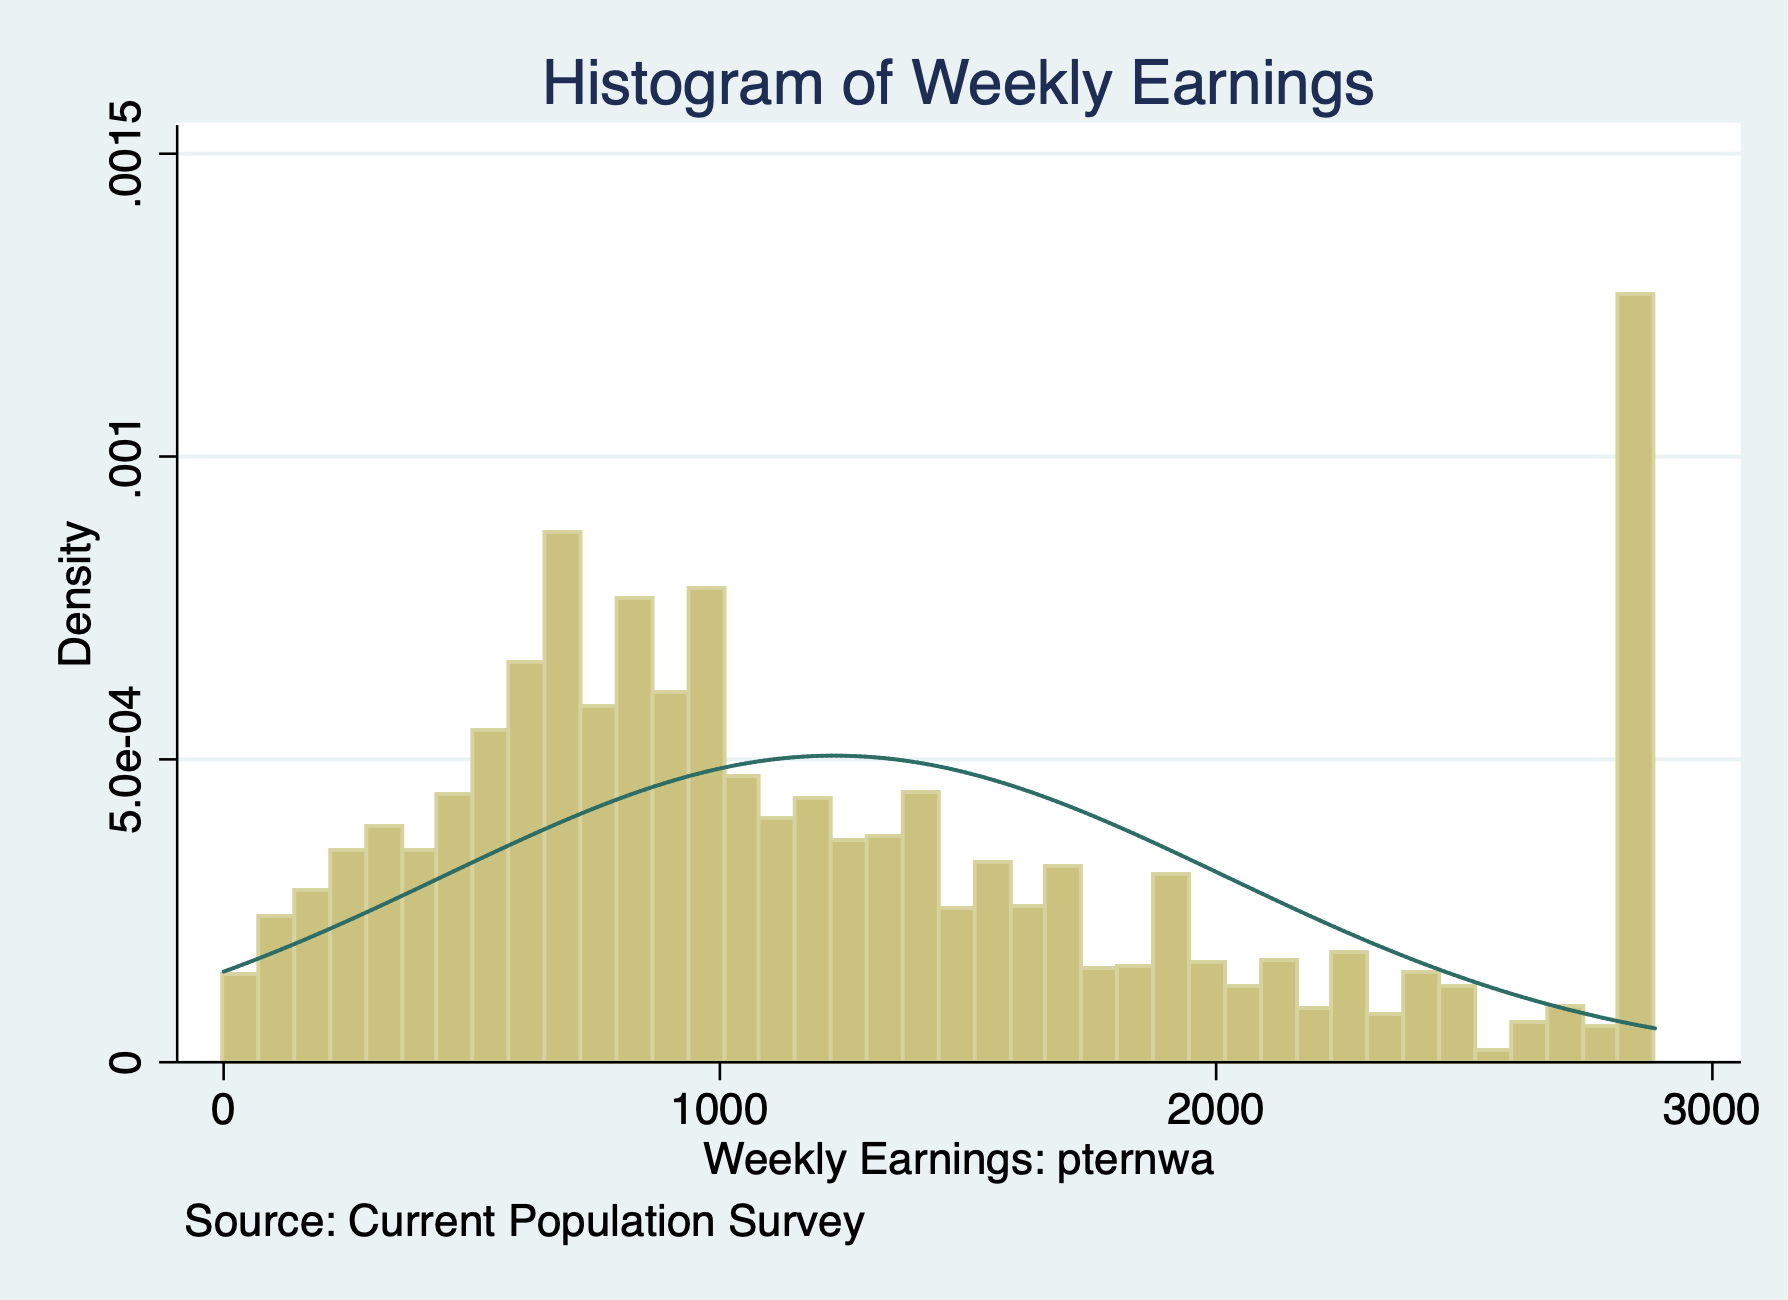
\includegraphics[keepaspectratio]{week9_histogram_earnings.png}}
\caption{Histogram of Earnings}
\end{figure}

Let us take a look at the natural log of earnings

\begin{Shaded}
\begin{Highlighting}[]
\KeywordTok{use} \StringTok{"/Users/Sam/Desktop/Econ 645/Data/CPS/jan2024.dta"}\NormalTok{, }\KeywordTok{clear}
\KeywordTok{sum}\NormalTok{ lnearnings, }\KeywordTok{detail}
\KeywordTok{histogram}\NormalTok{ lnearnings }\KeywordTok{if}\NormalTok{ prerelg==1, }\FunctionTok{normal} \BaseNTok{title}\NormalTok{(Histogram }\KeywordTok{of}\NormalTok{ LN Weekly Earnings) }\BaseNTok{caption}\NormalTok{(}\StringTok{"Source: Current Population Survey"}\NormalTok{)}
\KeywordTok{graph} \KeywordTok{export} \StringTok{"/Users/Sam/Desktop/Econ 645/R Markdown/week9\_histogram\_lnearnings.png"}\NormalTok{, }\KeywordTok{replace}
\end{Highlighting}
\end{Shaded}

\begin{verbatim}
               Natural Log of Weekly Earnings
-------------------------------------------------------------
      Percentiles      Smallest
 1%     4.356709      -3.506558
 5%     5.420535      -3.506558
10%     5.886104      -3.506558       Obs              10,652
25%      6.49224         .48858       Sum of Wgt.      10,652

50%     6.907755                      Mean            6.86502
                        Largest       Std. Dev.      .8181897
75%     7.426549       7.967145
90%     7.898151       7.967145       Variance       .6694343
95%     7.967145       7.967145       Skewness      -1.791008
99%     7.967145       7.967145       Kurtosis       13.92768

(bin=40, start=-3.5065579, width=.28684257)

(file /Users/Sam/Desktop/Econ 645/R Markdown/week9_histogram_lnearnings.png written in PNG format)
\end{verbatim}

\pandocbounded{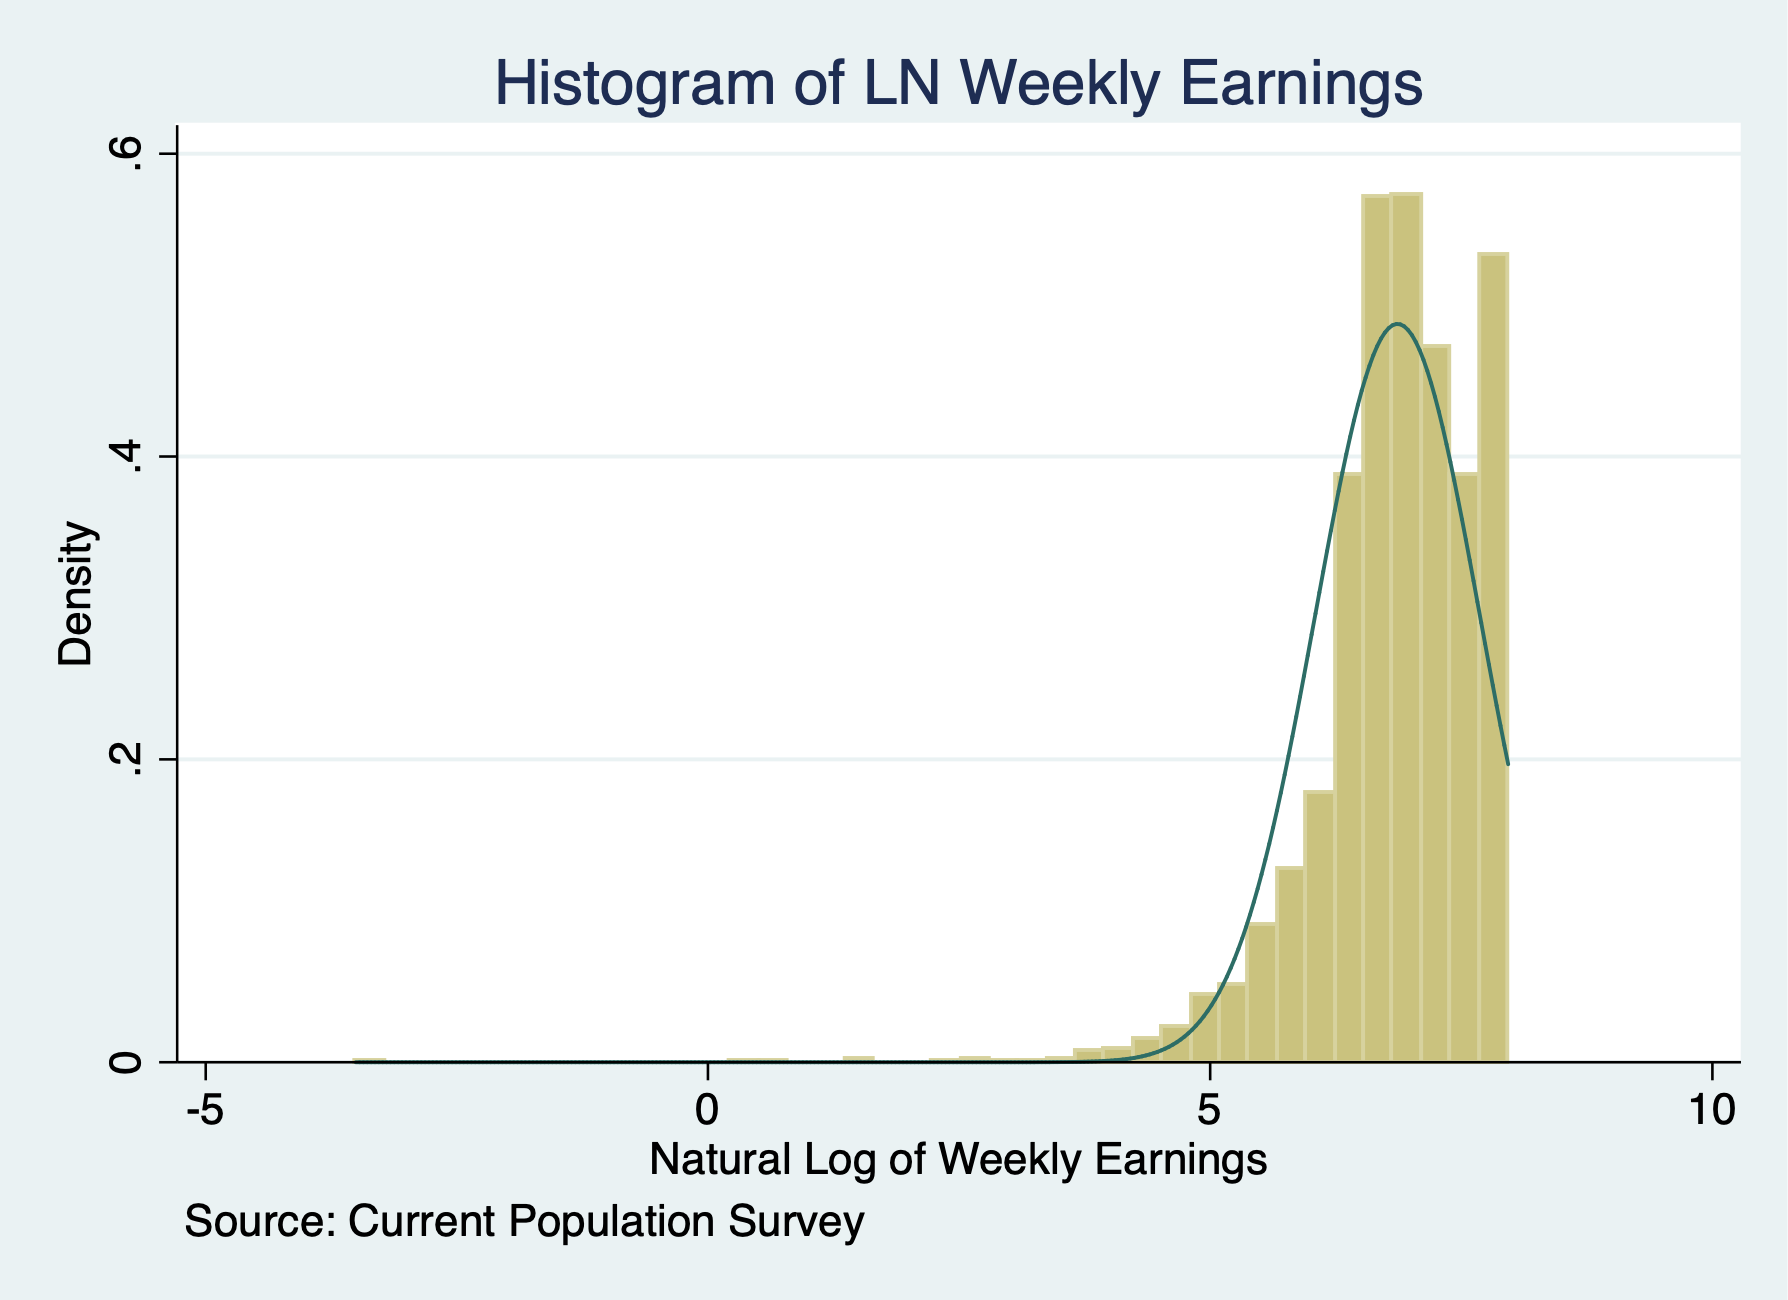
\includegraphics[keepaspectratio]{week9_histogram_lnearnings.png}}
We'll estimate the following Mincer Equation.
\[ ln(wwages_{i})=\beta_{0} + \beta_{1} edu_{i} + \beta_{2} exp + \beta_{3} exp^2 \beta_{4} marital_{i} + \beta_{5} veteran_{i} + \beta_{6} union_{i} + \beta_{7} female_{i} + \beta_{8} race_{i} + u_{i} \]
We'll need to use the option, \emph{ul(right-censored-value)} with our Tobit estimator.

\begin{Shaded}
\begin{Highlighting}[]
\KeywordTok{sum}\NormalTok{ lnearnings, }\KeywordTok{detail}
\FunctionTok{return} \OtherTok{list}
\KeywordTok{local}\NormalTok{ maxval }\OtherTok{\textasciigrave{}r(max)\textquotesingle{}}
\KeywordTok{tobit}\NormalTok{ lnearnings i.edu }\FunctionTok{exp}\NormalTok{ expsq i.marital i.veteran i.}\KeywordTok{union}\NormalTok{ i.female i.race, ul(}\OtherTok{\textasciigrave{}maxval\textquotesingle{}}\NormalTok{)}
\end{Highlighting}
\end{Shaded}

\begin{verbatim}
               Natural Log of Weekly Earnings
-------------------------------------------------------------
      Percentiles      Smallest
 1%     4.356709      -3.506558
 5%     5.420535      -3.506558
10%     5.886104      -3.506558       Obs              10,652
25%      6.49224         .48858       Sum of Wgt.      10,652

50%     6.907755                      Mean            6.86502
                        Largest       Std. Dev.      .8181897
75%     7.426549       7.967145
90%     7.898151       7.967145       Variance       .6694343
95%     7.967145       7.967145       Skewness      -1.791008
99%     7.967145       7.967145       Kurtosis       13.92768


scalars:
                  r(N) =  10652
              r(sum_w) =  10652
               r(mean) =  6.865020483352663
                r(Var) =  .6694343494891623
                 r(sd) =  .8181896781854207
           r(skewness) =  -1.791007993978133
           r(kurtosis) =  13.92768307319675
                r(sum) =  73126.19818867257
                r(min) =  -3.506557897319982
                r(max) =  7.967144987828557
                 r(p1) =  4.356708826689592
                 r(p5) =  5.420534999272286
                r(p10) =  5.886104031450156
                r(p25) =  6.492239835020471
                r(p50) =  6.907755278982137
                r(p75) =  7.426549072397305
                r(p90) =  7.898151125863075
                r(p95) =  7.967144987828557
                r(p99) =  7.967144987828557



Tobit regression                                Number of obs     =     10,568
                                                LR chi2(17)       =    3843.62
                                                Prob > chi2       =     0.0000
Log likelihood = -11364.619                     Pseudo R2         =     0.1446

---------------------------------------------------------------------------------------------------------
                             lnearnings |      Coef.   Std. Err.      t    P>|t|     [95% Conf. Interval]
----------------------------------------+----------------------------------------------------------------
                                    edu |
                                HS/GED  |   .3303562   .0299199    11.04   0.000     .2717075    .3890048
                                    AA  |    .444737   .0351051    12.67   0.000     .3759243    .5135497
                                 BS/BA  |    .831706   .0318545    26.11   0.000     .7692652    .8941468
                              AdDegree  |   1.046186    .034142    30.64   0.000     .9792607     1.11311
                                        |
                                    exp |   .0575487    .002085    27.60   0.000     .0534617    .0616356
                                  expsq |  -.0009113   .0000337   -27.03   0.000    -.0009774   -.0008452
                                        |
                                marital |
            Divorced/Separated/Widowed  |  -.0461827   .0217659    -2.12   0.034    -.0888481   -.0035173
                         Never Married  |   -.129934   .0189855    -6.84   0.000    -.1671492   -.0927189
                                        |
                                veteran |
                               Veteran  |    .042753   .0333981     1.28   0.201    -.0227135    .1082196
                                        |
                                  union |
                                 Union  |   .0448454   .0236468     1.90   0.058    -.0015067    .0911975
                                        |
                                 female |
                                Female  |  -.3347149   .0143948   -23.25   0.000    -.3629314   -.3064983
                                        |
                         race_ethnicity |
                              NH Asian  |   .0550537   .0846217     0.65   0.515    -.1108209    .2209282
                              NH Black  |  -.0576148   .0829774    -0.69   0.487    -.2202662    .1050365
NH Native Hawaiian or Pacific Islander  |   .1314362   .1374275     0.96   0.339    -.1379477      .40082
                  Latino/a or Hispanic  |   .0166878   .0818777     0.20   0.839     -.143808    .1771836
                        NH Multiracial  |   .0902634   .0954831     0.95   0.345    -.0969015    .2774284
                              NH White  |   .0553029   .0803465     0.69   0.491    -.1021914    .2127972
                                        |
                                  _cons |   5.817179   .0897475    64.82   0.000     5.641257    5.993101
----------------------------------------+----------------------------------------------------------------
                                 /sigma |   .7138391   .0052104                      .7036258    .7240524
---------------------------------------------------------------------------------------------------------
             0  left-censored observations
         9,690     uncensored observations
           878 right-censored observations at lnearnings >= 7.967145
\end{verbatim}

We will compare OLS to the Censored Regression Model

\begin{Shaded}
\begin{Highlighting}[]
\KeywordTok{est} \KeywordTok{clear}
\NormalTok{eststo OLS: }\KeywordTok{quietly} \KeywordTok{reg}\NormalTok{ lnearnings i.edu }\FunctionTok{exp}\NormalTok{ expsq i.marital i.veteran i.}\KeywordTok{union}\NormalTok{ i.female i.race}
\NormalTok{eststo Tobit: }\KeywordTok{quietly} \KeywordTok{tobit}\NormalTok{ lnearnings i.edu }\FunctionTok{exp}\NormalTok{ expsq i.marital i.veteran i.}\KeywordTok{union}\NormalTok{ i.female i.race, ul(}\OtherTok{\textasciigrave{}maxval\textquotesingle{}}\NormalTok{)}

\NormalTok{esttab OLS Tobit, }\KeywordTok{drop}\NormalTok{(0.* 1.race* 1.mar* 1.edu) mtitle(}\StringTok{"OLS"} \StringTok{"Tobit"}\NormalTok{)}
\end{Highlighting}
\end{Shaded}

\begin{verbatim}
                      (1)             (2)   
                      OLS           Tobit   
--------------------------------------------
main                                        
2.edu               0.330***        0.330***
                  (11.77)         (11.04)   

3.edu               0.442***        0.445***
                  (13.48)         (12.67)   

4.edu               0.788***        0.832***
                  (26.50)         (26.11)   

5.edu               0.951***        1.046***
                  (30.01)         (30.64)   

exp                0.0558***       0.0575***
                  (28.73)         (27.60)   

expsq           -0.000887***    -0.000911***
                 (-28.27)        (-27.03)   

2.marital         -0.0389         -0.0462*  
                  (-1.92)         (-2.12)   

3.marital          -0.118***       -0.130***
                  (-6.66)         (-6.84)   

1.veteran          0.0412          0.0428   
                   (1.34)          (1.28)   

1.union            0.0670**        0.0448   
                   (3.05)          (1.90)   

1.female           -0.304***       -0.335***
                 (-22.81)        (-23.25)   

2.race_eth~y       0.0325          0.0551   
                   (0.41)          (0.65)   

3.race_eth~y      -0.0466         -0.0576   
                  (-0.60)         (-0.69)   

4.race_eth~y        0.135           0.131   
                   (1.05)          (0.96)   

5.race_eth~y       0.0232          0.0167   
                   (0.30)          (0.20)   

6.race_eth~y       0.0730          0.0903   
                   (0.82)          (0.95)   

7.race_eth~y       0.0549          0.0553   
                   (0.73)          (0.69)   

_cons               5.813***        5.817***
                  (69.47)         (64.82)   
--------------------------------------------
sigma                                       
_cons                               0.714***
                                 (137.00)   
--------------------------------------------
N                   10568           10568   
--------------------------------------------
t statistics in parentheses
* p<0.05, ** p<0.01, *** p<0.001
\end{verbatim}

\textbf{Interpretation} A very similar interpretation to OLS, but we need normality and homoskedasticity for unbiased estimator. We can use a log-linear interpretation without a scaling factor, so the returns to education would only require \((e^\beta -1)*100\) interpretation.

\section{Censored Regression Model - Duration analysis}\label{censored-regression-model---duration-analysis}

\textbf{Lesson: We can look at a censored data for duration analysis similar to Wooldridge's example.}

This differs from a top-coded data, which we can use a Tobit analysis that we just saw.

We can look at the duration of time in months between an arrests for inmates
in a North Carolina prison after being released from prison. We want to
evaluate a work program to see if it is effective in increasing duration
before recidivism occurs.

Note: 893 inmates have not been arrested during the period they were followed
These observations are censored. The censoring times differed among inmates
ranging from 70 to 81 months.

Our dependent variable duration (time in months) is transformed by natural logarithm.
We have a bunch of observations that recidivate between 70 and 81 months.

\begin{Shaded}
\begin{Highlighting}[]
\KeywordTok{use} \StringTok{"/Users/Sam/Desktop/Econ 645/Data/Wooldridge/recid.dta"}\NormalTok{, }\KeywordTok{clear}
\KeywordTok{tab}\NormalTok{ durat}
\end{Highlighting}
\end{Shaded}

We have a bunch of observations that are censored after 69 months (but not all)

\begin{Shaded}
\begin{Highlighting}[]
\KeywordTok{use} \StringTok{"/Users/Sam/Desktop/Econ 645/Data/Wooldridge/recid.dta"}\NormalTok{, }\KeywordTok{clear}
\KeywordTok{tab}\NormalTok{ durat cens}
\end{Highlighting}
\end{Shaded}

\begin{verbatim}
           |         cens
     durat |         0          1 |     Total
-----------+----------------------+----------
         1 |         8          0 |         8 
         2 |        15          0 |        15 
         3 |        14          0 |        14 
         4 |        13          0 |        13 
         5 |        16          0 |        16 
         6 |        18          0 |        18 
         7 |        18          0 |        18 
         8 |        16          0 |        16 
         9 |        18          0 |        18 
        10 |        22          0 |        22 
        11 |        11          0 |        11 
        12 |        14          0 |        14 
        13 |        15          0 |        15 
        14 |        16          0 |        16 
        15 |        23          0 |        23 
        16 |        11          0 |        11 
        17 |         9          0 |         9 
        18 |        16          0 |        16 
        19 |         9          0 |         9 
        20 |         8          0 |         8 
        21 |        13          0 |        13 
        22 |         7          0 |         7 
        23 |        16          0 |        16 
        24 |        12          0 |        12 
        25 |        13          0 |        13 
        26 |         8          0 |         8 
        27 |        11          0 |        11 
        28 |         9          0 |         9 
        29 |         8          0 |         8 
        30 |         7          0 |         7 
        31 |         6          0 |         6 
        32 |         6          0 |         6 
        33 |         6          0 |         6 
        34 |         4          0 |         4 
        35 |         5          0 |         5 
        36 |         6          0 |         6 
        37 |         6          0 |         6 
        38 |         4          0 |         4 
        39 |         4          0 |         4 
        40 |         2          0 |         2 
        41 |         7          0 |         7 
        42 |         5          0 |         5 
        43 |         5          0 |         5 
        44 |         4          0 |         4 
        45 |         4          0 |         4 
        46 |         7          0 |         7 
        47 |         4          0 |         4 
        48 |         1          0 |         1 
        49 |         4          0 |         4 
        50 |         5          0 |         5 
        51 |         2          0 |         2 
        52 |         2          0 |         2 
        53 |         8          0 |         8 
        54 |         3          0 |         3 
        55 |         5          0 |         5 
        56 |         2          0 |         2 
        57 |         4          0 |         4 
        58 |         1          0 |         1 
        59 |         5          0 |         5 
        60 |         3          0 |         3 
        62 |         3          0 |         3 
        63 |         2          0 |         2 
        64 |         1          0 |         1 
        65 |         2          0 |         2 
        66 |         3          0 |         3 
        67 |         3          0 |         3 
        68 |         4          0 |         4 
        69 |         2          0 |         2 
        70 |         2        103 |       105 
        71 |         2         88 |        90 
        72 |         1         84 |        85 
        73 |         1        107 |       108 
        74 |         1         71 |        72 
        75 |         0         44 |        44 
        76 |         0        105 |       105 
        77 |         1         60 |        61 
        78 |         0         54 |        54 
        79 |         0         60 |        60 
        80 |         0         69 |        69 
        81 |         0         48 |        48 
-----------+----------------------+----------
     Total |       552        893 |     1,445 
\end{verbatim}

We'll use the \emph{stset} command and set failure at cens==0. We'll use the \emph{stset} command to time set survival.

\begin{Shaded}
\begin{Highlighting}[]
\KeywordTok{use} \StringTok{"/Users/Sam/Desktop/Econ 645/Data/Wooldridge/recid.dta"}\NormalTok{, }\KeywordTok{clear}
\KeywordTok{stset}\NormalTok{ ldurat, failure(cens==0)}
\end{Highlighting}
\end{Shaded}

\begin{verbatim}
     failure event:  cens == 0
obs. time interval:  (0, ldurat]
 exit on or before:  failure

------------------------------------------------------------------------------
       1445  total observations
          8  observations end on or before enter()
------------------------------------------------------------------------------
       1437  observations remaining, representing
        544  failures in single-record/single-failure data
   5411.742  total analysis time at risk and under observation
                                                at risk from t =         0
                                     earliest observed entry t =         0
                                          last observed exit t =  4.394449
\end{verbatim}

We'll use the \emph{streg} command and set the distribution

\[ ldurat_i = \alpha + =\delta workprg_i + \beta_2 tserved_i + \beta_3 felon_i + \beta_4 alcohol_i + \beta_5 drugs_i + \beta_6 educ_i + x'_i \gamma + \varepsilon_i\]
Where \(x'\) are demographics of race, marital status, and age.

\begin{Shaded}
\begin{Highlighting}[]
\KeywordTok{streg}\NormalTok{ workprg priors tserved felon alcohol drugs }\BaseNTok{black}\NormalTok{ married educ age, dist(}\KeywordTok{weibull}\NormalTok{) nohr}
\end{Highlighting}
\end{Shaded}

\begin{verbatim}
     failure event:  cens == 0
obs. time interval:  (0, ldurat]
 exit on or before:  failure

------------------------------------------------------------------------------
       1445  total observations
          8  observations end on or before enter()
------------------------------------------------------------------------------
       1437  observations remaining, representing
        544  failures in single-record/single-failure data
   5411.742  total analysis time at risk and under observation
                                                at risk from t =         0
                                     earliest observed entry t =         0
                                          last observed exit t =  4.394449

         failure _d:  cens == 0
   analysis time _t:  ldurat

Fitting constant-only model:

Iteration 0:   log likelihood = -1254.5107
Iteration 1:   log likelihood = -1100.1536
Iteration 2:   log likelihood = -1079.1128
Iteration 3:   log likelihood = -1078.7957
Iteration 4:   log likelihood = -1078.7957

Fitting full model:

Iteration 0:   log likelihood = -1078.7957  
Iteration 1:   log likelihood = -1034.1821  
Iteration 2:   log likelihood = -1001.9186  
Iteration 3:   log likelihood = -1000.5996  
Iteration 4:   log likelihood = -1000.5919  
Iteration 5:   log likelihood = -1000.5919  

Weibull regression -- log relative-hazard form 

No. of subjects =        1,437                  Number of obs    =       1,437
No. of failures =          544
Time at risk    =  5411.742317
                                                LR chi2(10)      =      156.41
Log likelihood  =   -1000.5919                  Prob > chi2      =      0.0000

------------------------------------------------------------------------------
          _t |      Coef.   Std. Err.      z    P>|z|     [95% Conf. Interval]
-------------+----------------------------------------------------------------
     workprg |   .0780722    .091463     0.85   0.393    -.1011921    .2573364
      priors |   .0834203   .0139155     5.99   0.000     .0561465    .1106941
     tserved |   .0134545   .0016851     7.98   0.000     .0101519    .0167572
       felon |   -.287139    .106697    -2.69   0.007    -.4962614   -.0780167
     alcohol |   .4399456     .10658     4.13   0.000     .2310527    .6488385
       drugs |   .2920932   .0983695     2.97   0.003     .0992926    .4848938
       black |   .4515388   .0889883     5.07   0.000     .2771249    .6259527
     married |   -.146192   .1098131    -1.33   0.183    -.3614216    .0690377
        educ |   -.023948    .019578    -1.22   0.221    -.0623202    .0144241
         age |  -.0036431   .0005284    -6.89   0.000    -.0046788   -.0026073
       _cons |  -3.639277   .3077568   -11.83   0.000     -4.24247   -3.036085
-------------+----------------------------------------------------------------
       /ln_p |   .9214587   .0396737    23.23   0.000     .8436997    .9992178
-------------+----------------------------------------------------------------
           p |   2.512953   .0996982                      2.324953    2.716156
         1/p |   .3979381   .0157877                      .3681673    .4301163
------------------------------------------------------------------------------
\end{verbatim}

\textbf{Interpretation:}
Given the log-linear function form, we can easily determine the estimated percent change in duration before criminal recidivism.

\begin{Shaded}
\begin{Highlighting}[]
    \KeywordTok{display}\NormalTok{ (}\FunctionTok{exp}\NormalTok{(.0780722){-}1)*100}
\end{Highlighting}
\end{Shaded}

\begin{verbatim}
8.1200719
\end{verbatim}

Being a part of the work program increase the duration of time before recidivism, but it is not statistically significant.

\begin{Shaded}
\begin{Highlighting}[]
    \KeywordTok{display}\NormalTok{ (}\FunctionTok{exp}\NormalTok{({-}.287139){-}1)*100}
\end{Highlighting}
\end{Shaded}

\begin{verbatim}
-24.959259
\end{verbatim}

Being a felon reduces the duration of time before recidivism, where a felon has as 24\% decrease in duration of time before recidivism.

\chapter{Truncated Regression Models}\label{truncated-regression-models}

We will again look at the Janurary 2024 Current Population Survey data. However, we will truncate the data at \$2884 per week by dropping all observation at or above this threshold.

\section{Truncated Data}\label{truncated-data}

We will set the threshold \(c_i \geq 2884\). Every observation at or above this threshold will be dropped.

\begin{Shaded}
\begin{Highlighting}[]
\KeywordTok{use} \StringTok{"/Users/Sam/Desktop/Econ 645/Data/CPS/jan2024.dta"}\NormalTok{, }\KeywordTok{clear}
\KeywordTok{sum}\NormalTok{ earnings }\KeywordTok{if}\NormalTok{ prerelg==1, }\KeywordTok{detail}
\KeywordTok{est} \KeywordTok{clear}
\NormalTok{eststo OLS: }\KeywordTok{quietly} \KeywordTok{reg}\NormalTok{ lnearnings i.edu }\FunctionTok{exp}\NormalTok{ expsq i.marital i.veteran i.}\KeywordTok{union}\NormalTok{ i.female i.race }\KeywordTok{if}\NormalTok{ prerelg==1}
\KeywordTok{drop} \KeywordTok{if}\NormalTok{ earnings \textgreater{}= 2884}
\KeywordTok{sum}\NormalTok{ earnings }\KeywordTok{if}\NormalTok{ prerelg==1, }\KeywordTok{detail}
\end{Highlighting}
\end{Shaded}

\begin{verbatim}
                  Weekly Earnings: pternwa
-------------------------------------------------------------
      Percentiles      Smallest
 1%           70              0
 5%          225              0
10%          360              0       Obs              10,666
25%          656              0       Sum of Wgt.      10,666

50%         1000                      Mean           1230.474
                        Largest       Std. Dev.      788.1457
75%         1680        2884.61
90%       2692.3        2884.61       Variance       621173.7
95%      2884.61        2884.61       Skewness       .7779644
99%      2884.61        2884.61       Kurtosis       2.648218



(28,566 observations deleted)

                  Weekly Earnings: pternwa
-------------------------------------------------------------
      Percentiles      Smallest
 1%         62.5              0
 5%          206              0
10%          336              0       Obs               9,767
25%          620              0       Sum of Wgt.       9,767

50%          960                      Mean           1078.221
                        Largest       Std. Dev.      635.0599
75%         1450           2880
90%         2000           2880       Variance       403301.1
95%         2320           2880       Skewness       .7302792
99%         2780           2880       Kurtosis       2.975473
\end{verbatim}

Our largest value is now \$2880 weekly earnings, which is just below the threshold.

Let's look at a histogram of the truncated weekly earnings.

\begin{Shaded}
\begin{Highlighting}[]
\KeywordTok{histogram}\NormalTok{ earnings }\KeywordTok{if}\NormalTok{ prerelg, }\BaseNTok{title}\NormalTok{(}\StringTok{"Truncated Earnings"}\NormalTok{) }\KeywordTok{note}\NormalTok{(}\StringTok{"Source: Current Population Survey"}\NormalTok{)}
\KeywordTok{graph} \KeywordTok{export} \StringTok{"/Users/Sam/Desktop/Econ 645/Data/CPS/jan2024\_trunc.png"}\NormalTok{, }\KeywordTok{replace}
\end{Highlighting}
\end{Shaded}

\pandocbounded{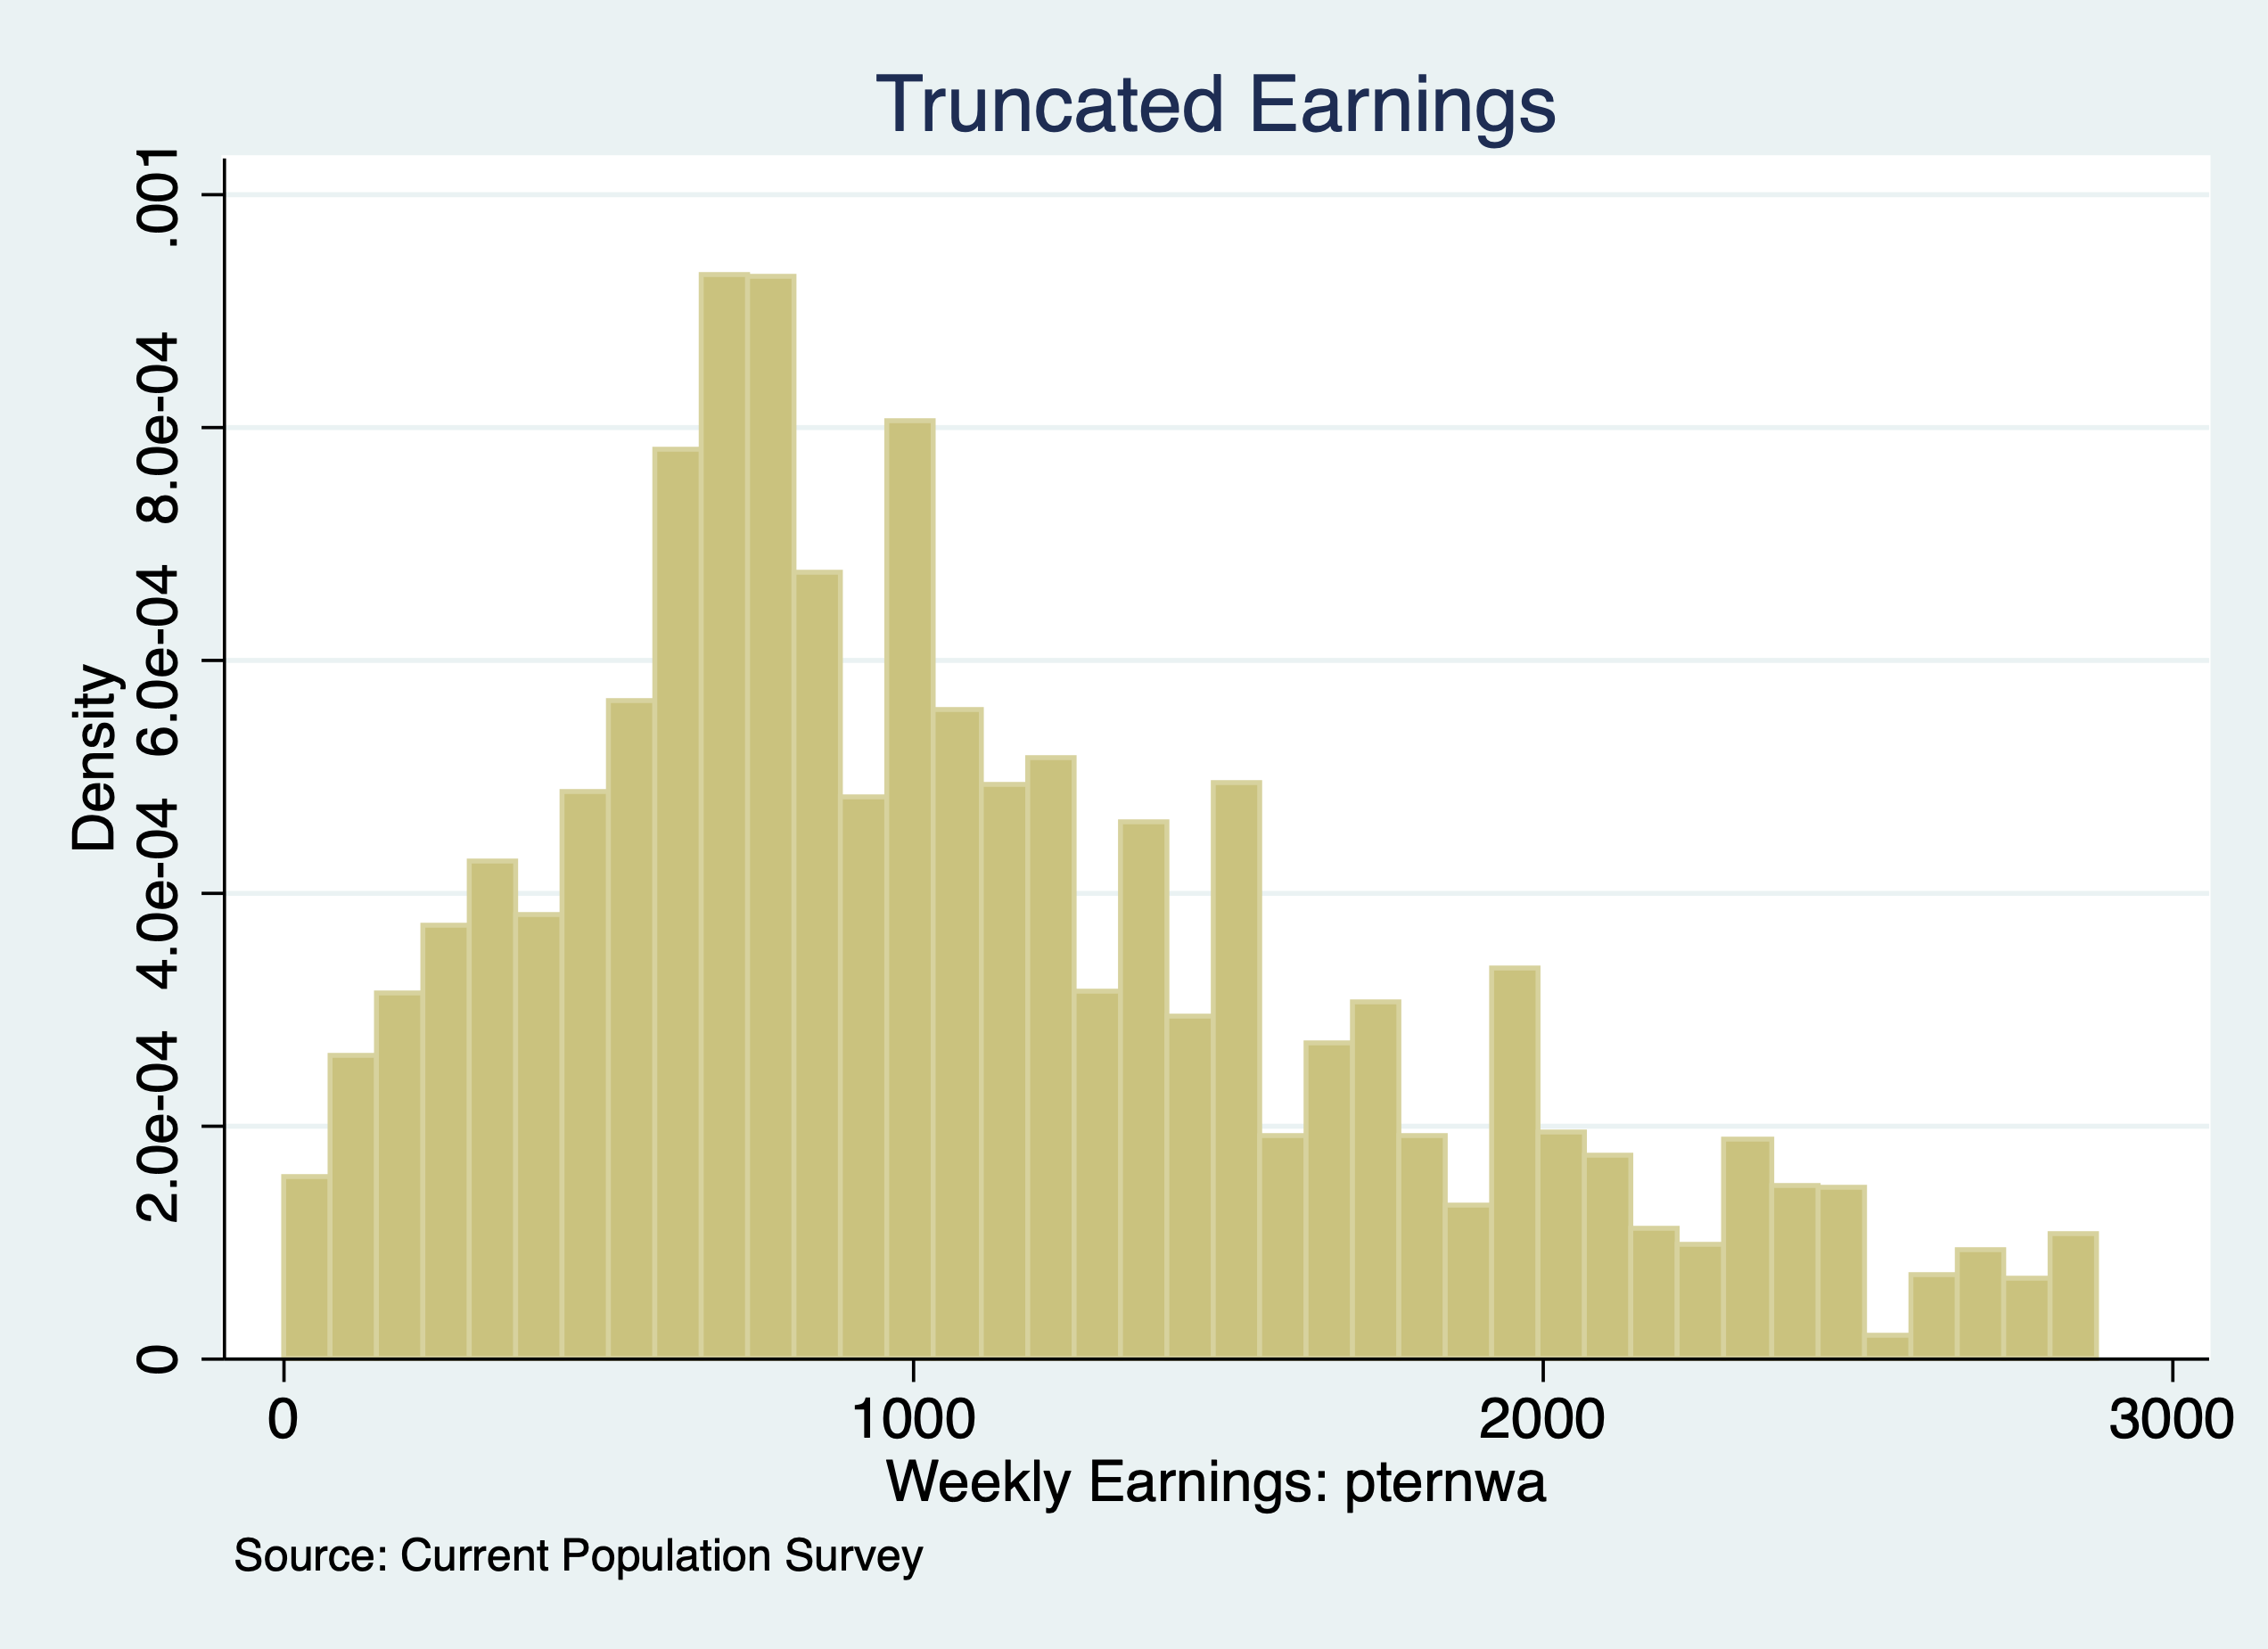
\includegraphics[keepaspectratio]{Week11_jan2024_trunc.png}}
We no longer have a spike in density at 2884 like we did with the censored data.

\section{Truncated Regression Models}\label{truncated-regression-models-1}

Next, we will use the command \emph{truncreg} and set the option \emph{ul()} at 2884.

\begin{Shaded}
\begin{Highlighting}[]
\NormalTok{eststo Truncated: }\KeywordTok{truncreg}\NormalTok{ lnearnings i.edu }\FunctionTok{exp}\NormalTok{ expsq i.marital i.veteran i.}\KeywordTok{union}\NormalTok{ i.female i.race, ul(2884)}
\end{Highlighting}
\end{Shaded}

\begin{verbatim}
(note: 0 obs. truncated)

Fitting full model:

Iteration 0:   log likelihood = -9654.7635  
Iteration 1:   log likelihood = -9654.7551  
Iteration 2:   log likelihood = -9654.7551  

Truncated regression
Limit:   lower =       -inf                     Number of obs =   =      9,669
         upper =       2884                     Wald chi2(17)     =    3276.34
Log likelihood = -9654.7551                     Prob > chi2       =     0.0000

---------------------------------------------------------------------------------------------------------
                             lnearnings |      Coef.   Std. Err.      z    P>|z|     [95% Conf. Interval]
----------------------------------------+----------------------------------------------------------------
                                    edu |
                                HS/GED  |   .3230896   .0276751    11.67   0.000     .2688475    .3773317
                                    AA  |   .4320131   .0325527    13.27   0.000     .3682109    .4958153
                                 BS/BA  |   .6971765   .0297669    23.42   0.000     .6388344    .7555186
                              AdDegree  |   .8088922   .0325213    24.87   0.000     .7451517    .8726327
                                        |
                                    exp |    .054815   .0019609    27.95   0.000     .0509716    .0586583
                                  expsq |  -.0008866   .0000319   -27.81   0.000    -.0009491   -.0008241
                                        |
                                marital |
            Divorced/Separated/Widowed  |  -.0290168   .0206418    -1.41   0.160    -.0694739    .0114404
                         Never Married  |  -.1028859   .0178986    -5.75   0.000    -.1379665   -.0678053
                                        |
                                veteran |
                               Veteran  |   .0280901   .0322307     0.87   0.383    -.0350809    .0912612
                                        |
                                  union |
                                 Union  |   .1126058   .0223161     5.05   0.000      .068867    .1563446
                                        |
                                 female |
                                Female  |  -.2718903   .0137518   -19.77   0.000    -.2988434   -.2449372
                                        |
                         race_ethnicity |
                              NH Asian  |  -.0426197   .0795044    -0.54   0.592    -.1984454    .1132061
                              NH Black  |    -.04673   .0774491    -0.60   0.546    -.1985275    .1050674
NH Native Hawaiian or Pacific Islander  |    .136987   .1278521     1.07   0.284    -.1135985    .3875724
                  Latino/a or Hispanic  |   .0151638    .076424     0.20   0.843    -.1346244     .164952
                        NH Multiracial  |   .0275207   .0898433     0.31   0.759     -.148569    .2036103
                              NH White  |    .035842   .0750013     0.48   0.633    -.1111579    .1828419
                                        |
                                  _cons |   5.814378   .0837643    69.41   0.000     5.650203    5.978553
----------------------------------------+----------------------------------------------------------------
                                 /sigma |   .6567763   .0047229   139.06   0.000     .6475195    .6660331
---------------------------------------------------------------------------------------------------------
\end{verbatim}

We can directly compare our OLS and Truncated Regression Model coefficients.

\begin{Shaded}
\begin{Highlighting}[]
\NormalTok{esttab OLS Truncated}
\end{Highlighting}
\end{Shaded}

\begin{verbatim}
                      (1)             (2)   
                      OLS             TRM   
--------------------------------------------
main                                        
1.edu                   0               0   
                      (.)             (.)   

2.edu               0.330***        0.323***
                  (11.77)         (11.67)   

3.edu               0.442***        0.432***
                  (13.48)         (13.27)   

4.edu               0.788***        0.697***
                  (26.50)         (23.42)   

5.edu               0.951***        0.809***
                  (30.01)         (24.87)   

exp                0.0558***       0.0548***
                  (28.73)         (27.95)   

expsq           -0.000887***    -0.000887***
                 (-28.27)        (-27.81)   

1.marital               0               0   
                      (.)             (.)   

2.marital         -0.0389         -0.0290   
                  (-1.92)         (-1.41)   

3.marital          -0.118***       -0.103***
                  (-6.66)         (-5.75)   

0.veteran               0               0   
                      (.)             (.)   

1.veteran          0.0412          0.0281   
                   (1.34)          (0.87)   

0.union                 0               0   
                      (.)             (.)   

1.union            0.0670**         0.113***
                   (3.05)          (5.05)   

0.female                0               0   
                      (.)             (.)   

1.female           -0.304***       -0.272***
                 (-22.81)        (-19.77)   

1.race_eth~y            0               0   
                      (.)             (.)   

2.race_eth~y       0.0325         -0.0426   
                   (0.41)         (-0.54)   

3.race_eth~y      -0.0466         -0.0467   
                  (-0.60)         (-0.60)   

4.race_eth~y        0.135           0.137   
                   (1.05)          (1.07)   

5.race_eth~y       0.0232          0.0152   
                   (0.30)          (0.20)   

6.race_eth~y       0.0730          0.0275   
                   (0.82)          (0.31)   

7.race_eth~y       0.0549          0.0358   
                   (0.73)          (0.48)   

_cons               5.813***        5.814***
                  (69.47)         (69.41)   
--------------------------------------------
sigma                                       
_cons                               0.657***
                                 (139.06)   
--------------------------------------------
N                   10568            9669   
--------------------------------------------
t statistics in parentheses
* p<0.05, ** p<0.01, *** p<0.001
\end{verbatim}

\textbf{Interpretation}: Our union wage premium is estimated to be \(((e^{0.067})-1)*100\% = 6.9\%\) with the OLS estimator, while our union wage premium is estimated to be
\(((e^{0.113})-1)*100\% = 12.0\%\).

We can see that our OLS estimates are biased upwards for education and experience, but downward biased for union wage premium.

Source: \url{https://stats.oarc.ucla.edu/stata/output/truncated-regression/}

\chapter{Sample Selection Correction}\label{sample-selection-correction}

\textbf{Lesson: Similar to tobit, when we don't account for the truncation of the data, or why certain parts of the population are not sampled, we will commit a type of omitted variable bias without our lambda(zy)-hat. We can use a Heckit method for sample selection correction.}

We want to see if there is sample selection bias due to unobservable wage offers
for non-working women.

\begin{enumerate}
\def\labelenumi{\arabic{enumi}.}
\item
  We need to estimate a logit or probit to test and correct for sample selection bias due to unobserved wage offer for nonworking women. Spousal income, education, experience, age, and number of kids less than 6.
  \[ ln(wages_{i})=\beta_{0}+ \mathbf{x'\beta} + u_{i} \]
  Where \(\mathbf{x}\) is a vector that includes education, experience, and experience squared
\item
  We use the Heckit command to implement a Heckman Method for sample selection correction.
\end{enumerate}

\[ ln(wages_{i})=\beta_{0}+ \mathbf{x'\beta} +\mathbf{z'\delta} + u_{i} \]
Where \(\mathbf{z}\) is a vector that includes spousal income, education, experience, age, and number of kids less than 6.

\section{OLS}\label{ols}

\begin{Shaded}
\begin{Highlighting}[]
\KeywordTok{use} \StringTok{"/Users/Sam/Desktop/Econ 645/Data/Wooldridge/mroz.dta"}\NormalTok{, }\KeywordTok{clear}
\KeywordTok{reg}\NormalTok{ lwage educ exper expersq    }
\end{Highlighting}
\end{Shaded}

\begin{verbatim}
      Source |       SS           df       MS      Number of obs   =       428
-------------+----------------------------------   F(3, 424)       =     26.29
       Model |  35.0222967         3  11.6740989   Prob > F        =    0.0000
    Residual |  188.305144       424  .444115906   R-squared       =    0.1568
-------------+----------------------------------   Adj R-squared   =    0.1509
       Total |  223.327441       427  .523015084   Root MSE        =    .66642

------------------------------------------------------------------------------
       lwage |      Coef.   Std. Err.      t    P>|t|     [95% Conf. Interval]
-------------+----------------------------------------------------------------
        educ |   .1074896   .0141465     7.60   0.000     .0796837    .1352956
       exper |   .0415665   .0131752     3.15   0.002     .0156697    .0674633
     expersq |  -.0008112   .0003932    -2.06   0.040    -.0015841   -.0000382
       _cons |  -.5220406   .1986321    -2.63   0.009    -.9124667   -.1316144
------------------------------------------------------------------------------
\end{verbatim}

\textbf{Notice:} an assumption is used to exclude spousal income, age, kids less than 6, and kids greater than 6 from our main regression.

\begin{Shaded}
\begin{Highlighting}[]
\KeywordTok{display}\NormalTok{ (}\FunctionTok{exp}\NormalTok{(\_b[educ]){-}1)*100}
\end{Highlighting}
\end{Shaded}

\begin{verbatim}
11.347933
\end{verbatim}

\section{Heckman Method - Heckit}\label{heckman-method---heckit}

We will use a subset of all exogenous variable
1. What are the factors correlated with being in the labor force?
2. What is the impact of education and experience on wages

\begin{Shaded}
\begin{Highlighting}[]
\KeywordTok{use} \StringTok{"/Users/Sam/Desktop/Econ 645/Data/Wooldridge/mroz.dta"}\NormalTok{, }\KeywordTok{clear}
\KeywordTok{heckman}\NormalTok{ lwage educ exper expersq, select(inlf=nwifeinc educ exper expersq age kidslt6 kidsge6) twostep }
\end{Highlighting}
\end{Shaded}

\begin{verbatim}
Heckman selection model -- two-step estimates   Number of obs     =        753
(regression model with sample selection)        Censored obs      =        325
                                                Uncensored obs    =        428

                                                Wald chi2(3)      =      51.53
                                                Prob > chi2       =     0.0000

------------------------------------------------------------------------------
             |      Coef.   Std. Err.      z    P>|z|     [95% Conf. Interval]
-------------+----------------------------------------------------------------
lwage        |
        educ |   .1090655    .015523     7.03   0.000     .0786411      .13949
       exper |   .0438873   .0162611     2.70   0.007     .0120163    .0757584
     expersq |  -.0008591   .0004389    -1.96   0.050    -.0017194    1.15e-06
       _cons |  -.5781032   .3050062    -1.90   0.058    -1.175904     .019698
-------------+----------------------------------------------------------------
inlf         |
    nwifeinc |  -.0120237   .0048398    -2.48   0.013    -.0215096   -.0025378
        educ |   .1309047   .0252542     5.18   0.000     .0814074     .180402
       exper |   .1233476   .0187164     6.59   0.000     .0866641    .1600311
     expersq |  -.0018871      .0006    -3.15   0.002     -.003063   -.0007111
         age |  -.0528527   .0084772    -6.23   0.000    -.0694678   -.0362376
     kidslt6 |  -.8683285   .1185223    -7.33   0.000    -1.100628    -.636029
     kidsge6 |    .036005   .0434768     0.83   0.408     -.049208    .1212179
       _cons |   .2700768    .508593     0.53   0.595    -.7267473    1.266901
-------------+----------------------------------------------------------------
mills        |
      lambda |   .0322619   .1336246     0.24   0.809    -.2296376    .2941613
-------------+----------------------------------------------------------------
         rho |    0.04861
       sigma |  .66362875
------------------------------------------------------------------------------
\end{verbatim}

\begin{Shaded}
\begin{Highlighting}[]
\KeywordTok{est} \KeywordTok{clear}
\NormalTok{eststo OLS: }\KeywordTok{reg}\NormalTok{ lwage educ exper expersq    }
\NormalTok{eststo Heckman: }\KeywordTok{heckman}\NormalTok{ lwage educ exper expersq, select(inlf=nwifeinc educ exper expersq age kidslt6 kidsge6) twostep }
\NormalTok{esttab, mtitle}
\end{Highlighting}
\end{Shaded}

\begin{verbatim}
                      (1)             (2)   
                      OLS         Heckman   
--------------------------------------------
main                                        
educ                0.107***        0.109***
                   (7.60)          (7.03)   

exper              0.0416**        0.0439** 
                   (3.15)          (2.70)   

expersq         -0.000811*      -0.000859   
                  (-2.06)         (-1.96)   

_cons              -0.522**        -0.578   
                  (-2.63)         (-1.90)   
--------------------------------------------
inlf                                        
nwifeinc                          -0.0120*  
                                  (-2.48)   

educ                                0.131***
                                   (5.18)   

exper                               0.123***
                                   (6.59)   

expersq                          -0.00189** 
                                  (-3.15)   

age                               -0.0529***
                                  (-6.23)   

kidslt6                            -0.868***
                                  (-7.33)   

kidsge6                            0.0360   
                                   (0.83)   

_cons                               0.270   
                                   (0.53)   
--------------------------------------------
mills                                       
lambda                             0.0323   
                                   (0.24)   
--------------------------------------------
N                     428             753   
--------------------------------------------
t statistics in parentheses
* p<0.05, ** p<0.01, *** p<0.001
\end{verbatim}

There is no real evidence of sample selection bias in the wage offer equation.
Our lambda-hat is not statistically significant and we fail to reject \(H_0: \rho=0\). Also, we notice very little difference between our OLS and Heckman Method.

\textbf{Interpretation:} we will have a similar interpretation to our OLS. We have a log-linear model so our interpretation of the return would be \(e^\beta\) or \((e^\beta-1)*100\). Our \(\hat{\lambda}\) would be a potential omitted variable, but our example shows that we fail to reject the null hypothesis and selection bias is does not appear to be problematic.

\chapter{Subgroup Functions Part II}\label{subgroup-functions-part-ii}

\section{Computing values within subgroups: Running sums}\label{computing-values-within-subgroups-running-sums}

As we mentioned earlier, when we use \emph{egen sum} vs \emph{gen sum}, we get different
results. \emph{Egen sum()} is similar to \emph{egen total()}, but it can be confusing.
When we use \emph{gen} with \emph{sum()}, we generate a \textbf{RUNNING} sum not a constant of total.

We can generate the tv running sum across all individuals over time

\begin{Shaded}
\begin{Highlighting}[]
\NormalTok{cd }\StringTok{"/Users/Sam/Desktop/Econ 645/Data/Mitchell"}
\KeywordTok{use}\NormalTok{ tv1, }\KeywordTok{clear}
\KeywordTok{generate}\NormalTok{ tvrunsum = }\KeywordTok{sum}\NormalTok{(tv)}
\end{Highlighting}
\end{Shaded}

\begin{verbatim}
/Users/Sam/Desktop/Econ 645/Data/Mitchell
\end{verbatim}

We can generate the tv running sum within an individuals time period

\begin{Shaded}
\begin{Highlighting}[]
\KeywordTok{bysort}\NormalTok{ kidid (dt): }\KeywordTok{generate}\NormalTok{ bytvrunsum=}\KeywordTok{sum}\NormalTok{(tv)}
\end{Highlighting}
\end{Shaded}

We can generate the total sum with an individuals time period

\begin{Shaded}
\begin{Highlighting}[]
\KeywordTok{bysort}\NormalTok{ kidid (dt): }\KeywordTok{egen}\NormalTok{ bytvsum=}\KeywordTok{total}\NormalTok{(tv)}
\end{Highlighting}
\end{Shaded}

We can generate the total sum for all individuals over time

\begin{Shaded}
\begin{Highlighting}[]
\KeywordTok{egen}\NormalTok{ tvsum = }\KeywordTok{total}\NormalTok{(tv)}
\end{Highlighting}
\end{Shaded}

We can also calculate a running average

\begin{Shaded}
\begin{Highlighting}[]
\KeywordTok{bysort}\NormalTok{ kidid (dt): }\KeywordTok{generate}\NormalTok{ bytvrunavg=}\KeywordTok{sum}\NormalTok{(tv)/}\DataTypeTok{\_n}
\end{Highlighting}
\end{Shaded}

We can compute the individual's average average

\begin{Shaded}
\begin{Highlighting}[]
\KeywordTok{bysort}\NormalTok{ kidid (dt): }\KeywordTok{egen}\NormalTok{ bytvavg = }\KeywordTok{mean}\NormalTok{(tv)}
\OtherTok{list}\NormalTok{ kidid tv tv* }\KeywordTok{by}\NormalTok{*, sepby(kidid)}
\end{Highlighting}
\end{Shaded}

\begin{verbatim}
     | kidid   tv   tv   tvrunsum   tvsum   bytvru~m   bytvsum   bytvrun~g   bytvavg |
     |-------------------------------------------------------------------------------|
  1. |     1    1    1          1      38          1         4           1         2 |
  2. |     1    3    3          4      38          4         4           2         2 |
     |-------------------------------------------------------------------------------|
  3. |     2    8    8         12      38          8         8           8         8 |
     |-------------------------------------------------------------------------------|
  4. |     3    2    2         14      38          2        14           2       3.5 |
  5. |     3    5    5         19      38          7        14         3.5       3.5 |
  6. |     3    1    1         20      38          8        14   2.6666667       3.5 |
  7. |     3    6    6         26      38         14        14         3.5       3.5 |
     |-------------------------------------------------------------------------------|
  8. |     4    7    7         33      38          7        12           7         4 |
  9. |     4    1    1         34      38          8        12           4         4 |
 10. |     4    4    4         38      38         12        12           4         4 |
     +-------------------------------------------------------------------------------+
\end{verbatim}

\section{Computing values within subgroups: More examples}\label{computing-values-within-subgroups-more-examples}

There are other useful calculations we can do with subscripting/indexing.
Some do overlap with egen, but it is helpful to know the differences.

\subsection*{Counting}\label{counting}
\addcontentsline{toc}{subsection}{Counting}

Count the number of observations: this can be done with subscripting or egen
depending upon what we want

\begin{Shaded}
\begin{Highlighting}[]
\NormalTok{cd }\StringTok{"/Users/Sam/Desktop/Econ 645/Data/Mitchell"}
\KeywordTok{use}\NormalTok{ tv1, }\KeywordTok{clear}

\NormalTok{*Generate }\KeywordTok{total}\NormalTok{ observation }\FunctionTok{count}\NormalTok{ per individual }\FunctionTok{missing} \KeywordTok{or} \KeywordTok{not} \FunctionTok{missing}\NormalTok{:}
\KeywordTok{bysort}\NormalTok{ kidid (dt): }\KeywordTok{generate}\NormalTok{ idcount=\_N}

\NormalTok{*Generate the }\KeywordTok{total}\NormalTok{ observation without }\FunctionTok{missing}
\KeywordTok{bysort}\NormalTok{ kidid (dt): }\KeywordTok{egen}\NormalTok{ idcount\_nomiss = }\FunctionTok{count}\NormalTok{(tv)}

\NormalTok{*Generate a running }\FunctionTok{count} \KeywordTok{of}\NormalTok{ an observation}
\KeywordTok{bysort}\NormalTok{ kidid (dt): }\KeywordTok{gen}\NormalTok{ idruncount = }\DataTypeTok{\_n}
\OtherTok{list}\NormalTok{, sepby(kidid)}
\end{Highlighting}
\end{Shaded}

\begin{verbatim}
/Users/Sam/Desktop/Econ 645/Data/Mitchell

     +----------------------------------------------------------------------------+
     | kidid          dt   female   wt   tv   vac   idcount   idcoun~s   idrunc~t |
     |----------------------------------------------------------------------------|
  1. |     1   07jan2002        1   53    1     1         2          2          1 |
  2. |     1   08jan2002        1   55    3     1         2          2          2 |
     |----------------------------------------------------------------------------|
  3. |     2   16jan2002        1   58    8     1         1          1          1 |
     |----------------------------------------------------------------------------|
  4. |     3   18jan2002        0   60    2     0         4          4          1 |
  5. |     3   19jan2002        0   63    5     1         4          4          2 |
  6. |     3   21jan2002        0   66    1     1         4          4          3 |
  7. |     3   22jan2002        0   64    6     0         4          4          4 |
     |----------------------------------------------------------------------------|
  8. |     4   10jan2002        1   62    7     0         3          3          1 |
  9. |     4   11jan2002        1   58    1     0         3          3          2 |
 10. |     4   13jan2002        1   55    4     0         3          3          3 |
     +----------------------------------------------------------------------------+
\end{verbatim}

\subsection*{Generate Binaries}\label{generate-binaries}
\addcontentsline{toc}{subsection}{Generate Binaries}

We can generate binary variables to find first and last observations or nth
observation. This differences from id counts, we are generating binaries for
when the qualifier is true.

\begin{Shaded}
\begin{Highlighting}[]
\NormalTok{cd }\StringTok{"/Users/Sam/Desktop/Econ 645/Data/Mitchell"}
\KeywordTok{use}\NormalTok{ tv1, }\KeywordTok{clear}

\NormalTok{*Find individuals with only one observation}
\KeywordTok{bysort}\NormalTok{ kidid (dt): }\KeywordTok{generate}\NormalTok{ singleob = (\_N==1)}

\NormalTok{*Find the first observation }\KeywordTok{of}\NormalTok{ an individual}
\KeywordTok{bysort}\NormalTok{ kidid (dt): }\KeywordTok{generate}\NormalTok{ firstob = (}\DataTypeTok{\_n}\NormalTok{==1)}

\NormalTok{*Find the }\FunctionTok{last}\NormalTok{ observation }\KeywordTok{of}\NormalTok{ an individual }
\KeywordTok{bysort}\NormalTok{ kidid (dt): }\KeywordTok{generate}\NormalTok{ lastob = (}\DataTypeTok{\_n}\NormalTok{==\_N)}
\OtherTok{list}\NormalTok{, sepby(kidid)}
\end{Highlighting}
\end{Shaded}

\begin{verbatim}
/Users/Sam/Desktop/Econ 645/Data/Mitchell

     +--------------------------------------------------------------------------+
     | kidid          dt   female   wt   tv   vac   singleob   firstob   lastob |
     |--------------------------------------------------------------------------|
  1. |     1   07jan2002        1   53    1     1          0         1        0 |
  2. |     1   08jan2002        1   55    3     1          0         0        1 |
     |--------------------------------------------------------------------------|
  3. |     2   16jan2002        1   58    8     1          1         1        1 |
     |--------------------------------------------------------------------------|
  4. |     3   18jan2002        0   60    2     0          0         1        0 |
  5. |     3   19jan2002        0   63    5     1          0         0        0 |
  6. |     3   21jan2002        0   66    1     1          0         0        0 |
  7. |     3   22jan2002        0   64    6     0          0         0        1 |
     |--------------------------------------------------------------------------|
  8. |     4   10jan2002        1   62    7     0          0         1        0 |
  9. |     4   11jan2002        1   58    1     0          0         0        0 |
 10. |     4   13jan2002        1   55    4     0          0         0        1 |
     +--------------------------------------------------------------------------+
\end{verbatim}

We can create binaries depending upon leads and lags too.
Look for a change in vac

\begin{Shaded}
\begin{Highlighting}[]
\NormalTok{cd }\StringTok{"/Users/Sam/Desktop/Econ 645/Data/Mitchell"}
\KeywordTok{use}\NormalTok{ tv1, }\KeywordTok{clear}
\KeywordTok{bysort}\NormalTok{ kidid (dt): }\KeywordTok{generate}\NormalTok{ vacstart=(vac==1) \& (vac[}\DataTypeTok{\_n}\NormalTok{{-}1]==0)}
\KeywordTok{bysort}\NormalTok{ kidid (dt): }\KeywordTok{generate}\NormalTok{ vacend=(vac==1) \& (vac[}\DataTypeTok{\_n}\NormalTok{+1]==0)}
\OtherTok{list}\NormalTok{ kidid dt vac*, sepby(kidid)}
\end{Highlighting}
\end{Shaded}

\begin{verbatim}
/Users/Sam/Desktop/Econ 645/Data/Mitchell

     +---------------------------------------------+
     | kidid          dt   vac   vacstart   vacend |
     |---------------------------------------------|
  1. |     1   07jan2002     1          0        0 |
  2. |     1   08jan2002     1          0        0 |
     |---------------------------------------------|
  3. |     2   16jan2002     1          0        0 |
     |---------------------------------------------|
  4. |     3   18jan2002     0          0        0 |
  5. |     3   19jan2002     1          1        0 |
  6. |     3   21jan2002     1          0        1 |
  7. |     3   22jan2002     0          0        0 |
     |---------------------------------------------|
  8. |     4   10jan2002     0          0        0 |
  9. |     4   11jan2002     0          0        0 |
 10. |     4   13jan2002     0          0        0 |
     +---------------------------------------------+
\end{verbatim}

\subsection*{Fill in Missing}\label{fill-in-missing}
\addcontentsline{toc}{subsection}{Fill in Missing}

Another useful tool that we should use with caution is filling in missings.
This should only really be applied when we have a constant variable that
does not change over time.

\begin{Shaded}
\begin{Highlighting}[]
\NormalTok{cd }\StringTok{"/Users/Sam/Desktop/Econ 645/Data/Mitchell"}
\KeywordTok{use}\NormalTok{ tv2, }\KeywordTok{clear}
\KeywordTok{sort}\NormalTok{ kidid dt}
\OtherTok{list}\NormalTok{, sepby(kidid)}
\end{Highlighting}
\end{Shaded}

\begin{verbatim}
/Users/Sam/Desktop/Econ 645/Data/Mitchell

     +--------------------------------------------+
     | kidid          dt   female   wt   tv   vac |
     |--------------------------------------------|
  1. |     1   07jan2002        1   53    1     1 |
  2. |     1   08jan2002        1   55    3     1 |
     |--------------------------------------------|
  3. |     2   16jan2002        1   58    8     1 |
     |--------------------------------------------|
  4. |     3   18jan2002        0   60    2     0 |
  5. |     3   19jan2002        0    .    .     . |
  6. |     3   21jan2002        0   66    .     1 |
  7. |     3   22jan2002        0   64    6     0 |
     |--------------------------------------------|
  8. |     4   10jan2002        1   62    7     0 |
  9. |     4   11jan2002        1   58    .     . |
 10. |     4   13jan2002        1    .    4     0 |
     +--------------------------------------------+
\end{verbatim}

We can backfill the observation with the last nonmissing observation.
First generate a copy of the variable with missing values.

\begin{Shaded}
\begin{Highlighting}[]
\KeywordTok{generate}\NormalTok{ tvimp1 = tv}
\KeywordTok{bysort}\NormalTok{ kidid (dt): }\KeywordTok{replace}\NormalTok{ tvimp1 = tv[}\DataTypeTok{\_n}\NormalTok{{-}1] }\KeywordTok{if} \FunctionTok{missing}\NormalTok{(tv)}
\OtherTok{list}\NormalTok{ kidid dt tv tvimp1, sepby(kidid)}
\end{Highlighting}
\end{Shaded}

\begin{verbatim}
(3 missing values generated)

(2 real changes made)

     +---------------------------------+
     | kidid          dt   tv   tvimp1 |
     |---------------------------------|
  1. |     1   07jan2002    1        1 |
  2. |     1   08jan2002    3        3 |
     |---------------------------------|
  3. |     2   16jan2002    8        8 |
     |---------------------------------|
  4. |     3   18jan2002    2        2 |
  5. |     3   19jan2002    .        2 |
  6. |     3   21jan2002    .        . |
  7. |     3   22jan2002    6        6 |
     |---------------------------------|
  8. |     4   10jan2002    7        7 |
  9. |     4   11jan2002    .        7 |
 10. |     4   13jan2002    4        4 |
     +---------------------------------+
\end{verbatim}

Notice that we are still missing the 3rd observation for the 3rd kid.
It cannot backfill the 3rd observation from the second observation, since
the second observation is missing. There are a couple of strategies to use
We can generate a new variable like Mitchell.

\begin{Shaded}
\begin{Highlighting}[]
\KeywordTok{generate}\NormalTok{ tvimp2 = tvimp1}
\KeywordTok{bysort}\NormalTok{ kidid (dt): }\KeywordTok{replace}\NormalTok{ tvimp2 = tvimp2[}\DataTypeTok{\_n}\NormalTok{{-}1] }\KeywordTok{if} \FunctionTok{missing}\NormalTok{(tvimp2)}
\OtherTok{list}\NormalTok{ kidid tv tvimp*, sepby(kidid)}
\end{Highlighting}
\end{Shaded}

\begin{verbatim}
(1 missing value generated)

(1 real change made)

     +------------------------------+
     | kidid   tv   tvimp1   tvimp2 |
     |------------------------------|
  1. |     1    1        1        1 |
  2. |     1    3        3        3 |
     |------------------------------|
  3. |     2    8        8        8 |
     |------------------------------|
  4. |     3    2        2        2 |
  5. |     3    .        2        2 |
  6. |     3    .        .        2 |
  7. |     3    6        6        6 |
     |------------------------------|
  8. |     4    7        7        7 |
  9. |     4    .        7        7 |
 10. |     4    4        4        4 |
     +------------------------------+
\end{verbatim}

You can just replace tvimp1 twice instead of generating a new variable, but
that is up to the user. You would use tv{[}\_n-1{]} for the first replace and
tvimp1{[}\_n-1{]} for the second replace.

\subsection*{Interpolation}\label{interpolation}
\addcontentsline{toc}{subsection}{Interpolation}

We may need to interpolate between 2 known values and assume a linear trend.

\begin{Shaded}
\begin{Highlighting}[]
\KeywordTok{generate}\NormalTok{ tvimp3=tv}
\NormalTok{*Interpolate }\KeywordTok{for}\NormalTok{ 1 }\FunctionTok{missing} \OtherTok{value}\NormalTok{ between }\KeywordTok{two}\NormalTok{ known }\KeywordTok{values}
\KeywordTok{bysort}\NormalTok{ kidid (dt): }\KeywordTok{replace}\NormalTok{ tvimp3 = (tv[}\DataTypeTok{\_n}\NormalTok{{-}1]+tv[}\DataTypeTok{\_n}\NormalTok{+1])/2 }\KeywordTok{if} \FunctionTok{missing}\NormalTok{(tv)}
\OtherTok{list}\NormalTok{ kidid tv tvimp3, sepby(kidid)}
\end{Highlighting}
\end{Shaded}

\begin{verbatim}
(3 missing values generated)

(1 real change made)

     +---------------------+
     | kidid   tv   tvimp3 |
     |---------------------|
  1. |     1    1        1 |
  2. |     1    3        3 |
     |---------------------|
  3. |     2    8        8 |
     |---------------------|
  4. |     3    2        2 |
  5. |     3    .        . |
  6. |     3    .        . |
  7. |     3    6        6 |
     |---------------------|
  8. |     4    7        7 |
  9. |     4    .      5.5 |
 10. |     4    4        4 |
     +---------------------+
\end{verbatim}

This is a bit of hard coding, but you can interpolate with more than 1 missing.

\begin{Shaded}
\begin{Highlighting}[]
\KeywordTok{bysort}\NormalTok{ kidid (dt): }\KeywordTok{replace}\NormalTok{ tvimp3 = ((tvimp3[4]{-}tvimp3[1])/3)+tvimp3[}\DataTypeTok{\_n}\NormalTok{{-}1] }\KeywordTok{if} \FunctionTok{missing}\NormalTok{(tvimp3) \& kidid==3}
\OtherTok{list}\NormalTok{ kidid tv tvimp3, sepby(kidid)}
\end{Highlighting}
\end{Shaded}

\begin{verbatim}
(2 real changes made)

     +------------------------+
     | kidid   tv      tvimp3 |
     |------------------------|
  1. |     1    1           1 |
  2. |     1    3           3 |
     |------------------------|
  3. |     2    8           8 |
     |------------------------|
  4. |     3    2           2 |
  5. |     3    .   3.3333333 |
  6. |     3    .   4.6666667 |
  7. |     3    6           6 |
     |------------------------|
  8. |     4    7           7 |
  9. |     4    .         5.5 |
 10. |     4    4           4 |
     +------------------------+
\end{verbatim}

\subsection*{Indicators}\label{indicators}
\addcontentsline{toc}{subsection}{Indicators}

What is we want to find outliers in time-varying differences? We can generate
indicators variables to find when a variable changes more than a set limit.
For example we want to know if the tv viewing habits drop more than 2 hours

\begin{Shaded}
\begin{Highlighting}[]
\NormalTok{cd }\StringTok{"/Users/Sam/Desktop/Econ 645/Data/Mitchell"}
\KeywordTok{use}\NormalTok{ tv1, }\KeywordTok{clear}
\KeywordTok{bysort}\NormalTok{ kidid (dt): }\KeywordTok{generate}\NormalTok{ tvchange = tv[}\DataTypeTok{\_n}\NormalTok{]{-}tv[}\DataTypeTok{\_n}\NormalTok{{-}1]}
\KeywordTok{bysort}\NormalTok{ kidid (dt): }\KeywordTok{generate}\NormalTok{ tvchangerate = ((tv[}\DataTypeTok{\_n}\NormalTok{]{-}tv[}\DataTypeTok{\_n}\NormalTok{{-}1])/tv[}\DataTypeTok{\_n}\NormalTok{{-}1])}
\OtherTok{list}\NormalTok{, sepby(kidid)}
\end{Highlighting}
\end{Shaded}

\begin{verbatim}
/Users/Sam/Desktop/Econ 645/Data/Mitchell


(4 missing values generated)

(4 missing values generated)

     +--------------------------------------------------------------------+
     | kidid          dt   female   wt   tv   vac   tvchange   tvchange~e |
     |--------------------------------------------------------------------|
  1. |     1   07jan2002        1   53    1     1          .            . |
  2. |     1   08jan2002        1   55    3     1          2            2 |
     |--------------------------------------------------------------------|
  3. |     2   16jan2002        1   58    8     1          .            . |
     |--------------------------------------------------------------------|
  4. |     3   18jan2002        0   60    2     0          .            . |
  5. |     3   19jan2002        0   63    5     1          3          1.5 |
  6. |     3   21jan2002        0   66    1     1         -4          -.8 |
  7. |     3   22jan2002        0   64    6     0          5            5 |
     |--------------------------------------------------------------------|
  8. |     4   10jan2002        1   62    7     0          .            . |
  9. |     4   11jan2002        1   58    1     0         -6   -.85714286 |
 10. |     4   13jan2002        1   55    4     0          3            3 |
     +--------------------------------------------------------------------+
\end{verbatim}

Generate an indicator variable to see if tvchange is less than -2. This is not
very helpful with small datasets, but it is important with larger datasets such as the CPS.

\begin{Shaded}
\begin{Highlighting}[]
\KeywordTok{gen}\NormalTok{ tvchangeid=(tvchange \textless{}= {-}2) }\KeywordTok{if}\NormalTok{ !}\FunctionTok{missing}\NormalTok{(tvchange)}
\OtherTok{list}\NormalTok{, sepby(kidid)}
\end{Highlighting}
\end{Shaded}

\begin{verbatim}
(4 missing values generated)

     +-------------------------------------------------------------------------------+
     | kidid          dt   female   wt   tv   vac   tvchange   tvchange~e   tvchan~d |
     |-------------------------------------------------------------------------------|
  1. |     1   07jan2002        1   53    1     1          .            .          . |
  2. |     1   08jan2002        1   55    3     1          2            2          0 |
     |-------------------------------------------------------------------------------|
  3. |     2   16jan2002        1   58    8     1          .            .          . |
     |-------------------------------------------------------------------------------|
  4. |     3   18jan2002        0   60    2     0          .            .          . |
  5. |     3   19jan2002        0   63    5     1          3          1.5          0 |
  6. |     3   21jan2002        0   66    1     1         -4          -.8          1 |
  7. |     3   22jan2002        0   64    6     0          5            5          0 |
     |-------------------------------------------------------------------------------|
  8. |     4   10jan2002        1   62    7     0          .            .          . |
  9. |     4   11jan2002        1   58    1     0         -6   -.85714286          1 |
 10. |     4   13jan2002        1   55    4     0          3            3          0 |
     +-------------------------------------------------------------------------------+
\end{verbatim}

\section{Comparing the by, tsset, xtset commands}\label{comparing-the-by-tsset-xtset-commands}

Another way to find differences within vectors, we can use the tsset or xtset
command to establish the times series (tsset) or panel data (xtset).
We can use our bysort with subscripting/indexing.

\begin{Shaded}
\begin{Highlighting}[]
\NormalTok{cd }\StringTok{"/Users/Sam/Desktop/Econ 645/Data/Mitchell"}
\KeywordTok{use}\NormalTok{ tv1, }\KeywordTok{clear}
\KeywordTok{bysort}\NormalTok{ kidid (dt): }\KeywordTok{generate}\NormalTok{ ltv = tv[}\DataTypeTok{\_n}\NormalTok{{-}1]}
\OtherTok{list}\NormalTok{, sepby(kidid)}
\end{Highlighting}
\end{Shaded}

\begin{verbatim}
/Users/Sam/Desktop/Econ 645/Data/Mitchell


(4 missing values generated)

     +--------------------------------------------------+
     | kidid          dt   female   wt   tv   vac   ltv |
     |--------------------------------------------------|
  1. |     1   07jan2002        1   53    1     1     . |
  2. |     1   08jan2002        1   55    3     1     1 |
     |--------------------------------------------------|
  3. |     2   16jan2002        1   58    8     1     . |
     |--------------------------------------------------|
  4. |     3   18jan2002        0   60    2     0     . |
  5. |     3   19jan2002        0   63    5     1     2 |
  6. |     3   21jan2002        0   66    1     1     5 |
  7. |     3   22jan2002        0   64    6     0     1 |
     |--------------------------------------------------|
  8. |     4   10jan2002        1   62    7     0     . |
  9. |     4   11jan2002        1   58    1     0     7 |
 10. |     4   13jan2002        1   55    4     0     1 |
     +--------------------------------------------------+
\end{verbatim}

\subsection*{tsset}\label{tsset}
\addcontentsline{toc}{subsection}{tsset}

Instead we can establish a time series with \emph{tsset}

We'll need to specify that our cross-sectional groups is kidid.
We'll need to specify our date variable with dt.
We'll need to use the option, daily, to specify that time period is daily
as opposed to weeks, months, years. Or we can specify delta(1) for one day.

We can use the operator \emph{L.var} to specify that we want to a lag of 1 day

\begin{Shaded}
\begin{Highlighting}[]
\NormalTok{cd }\StringTok{"/Users/Sam/Desktop/Econ 645/Data/Mitchell"}
\KeywordTok{use}\NormalTok{ tv1, }\KeywordTok{clear}
\KeywordTok{sort}\NormalTok{ kidid dt}
\KeywordTok{tsset}\NormalTok{ kidid dt, }\FunctionTok{daily}\NormalTok{ delta(1)}
\KeywordTok{generate}\NormalTok{ lagtv = L.tv}
\end{Highlighting}
\end{Shaded}

\begin{verbatim}
/Users/Sam/Desktop/Econ 645/Data/Mitchell

       panel variable:  kidid (unbalanced)
        time variable:  dt, 07jan2002 to 22jan2002, but with gaps
                delta:  1 day

(6 missing values generated)
\end{verbatim}

We can use the operator F.var to specify that we want a lead of 1 day

\begin{Shaded}
\begin{Highlighting}[]
\KeywordTok{generate}\NormalTok{ leadtv = }\FunctionTok{F}\NormalTok{.tv}
\OtherTok{list}\NormalTok{, sepby(kidid)}
\end{Highlighting}
\end{Shaded}

\begin{verbatim}
(6 missing values generated)

     +-------------------------------------------------------------+
     | kidid          dt   female   wt   tv   vac   lagtv   leadtv |
     |-------------------------------------------------------------|
  1. |     1   07jan2002        1   53    1     1       .        3 |
  2. |     1   08jan2002        1   55    3     1       1        . |
     |-------------------------------------------------------------|
  3. |     2   16jan2002        1   58    8     1       .        . |
     |-------------------------------------------------------------|
  4. |     3   18jan2002        0   60    2     0       .        5 |
  5. |     3   19jan2002        0   63    5     1       2        . |
  6. |     3   21jan2002        0   66    1     1       .        6 |
  7. |     3   22jan2002        0   64    6     0       1        . |
     |-------------------------------------------------------------|
  8. |     4   10jan2002        1   62    7     0       .        1 |
  9. |     4   11jan2002        1   58    1     0       7        . |
 10. |     4   13jan2002        1   55    4     0       .        . |
     +-------------------------------------------------------------+
\end{verbatim}

\subsection*{xtset}\label{xtset}
\addcontentsline{toc}{subsection}{xtset}

We can establish a panel series with \emph{xtset}

We'll need to specify that our cross-sectional group is kidid.
We'll need to specify our time period is dt.
We'll use a delta of 1 to specify that the differnce is 1 day.
Or, we can use \emph{daily}, as well

Generate a lag with the l.var operator and generate a lead with the f.var

\begin{Shaded}
\begin{Highlighting}[]
\NormalTok{cd }\StringTok{"/Users/Sam/Desktop/Econ 645/Data/Mitchell"}
\KeywordTok{use}\NormalTok{ tv1, }\KeywordTok{clear}
\KeywordTok{sort}\NormalTok{ kidid dt}
\NormalTok{xtset kidid dt, }\FunctionTok{daily}\NormalTok{ delta(1)}
\KeywordTok{generate}\NormalTok{ lagtv = }\OtherTok{l}\NormalTok{.tv}
\KeywordTok{generate}\NormalTok{ leadtv = f.tv}
\end{Highlighting}
\end{Shaded}

\begin{verbatim}
/Users/Sam/Desktop/Econ 645/Data/Mitchell

       panel variable:  kidid (unbalanced)
        time variable:  dt, 07jan2002 to 22jan2002, but with gaps
                delta:  1 day

(6 missing values generated)

(6 missing values generated)
\end{verbatim}

What do you notice? You can see that there are some leads and lags missing.
Why? Because there is an unbalance panel and the daily differences cannot be
computed if we are missing days. In this case, we can use the bysort with
subscripting indexing

\begin{Shaded}
\begin{Highlighting}[]
\OtherTok{list}\NormalTok{, sepby(kidid)}
\KeywordTok{bysort}\NormalTok{ kidid (dt): }\KeywordTok{gen}\NormalTok{ bylagtv=tv[}\DataTypeTok{\_n}\NormalTok{{-}1]}
\KeywordTok{bysort}\NormalTok{ kidid (dt): }\KeywordTok{gen}\NormalTok{ byleadtv=tv[}\DataTypeTok{\_n}\NormalTok{+1]}
\OtherTok{list}\NormalTok{, sepby(kidid)}
\end{Highlighting}
\end{Shaded}

\begin{verbatim}
     | kidid          dt   female   wt   tv   vac   lagtv   leadtv |
     |-------------------------------------------------------------|
  1. |     1   07jan2002        1   53    1     1       .        3 |
  2. |     1   08jan2002        1   55    3     1       1        . |
     |-------------------------------------------------------------|
  3. |     2   16jan2002        1   58    8     1       .        . |
     |-------------------------------------------------------------|
  4. |     3   18jan2002        0   60    2     0       .        5 |
  5. |     3   19jan2002        0   63    5     1       2        . |
  6. |     3   21jan2002        0   66    1     1       .        6 |
  7. |     3   22jan2002        0   64    6     0       1        . |
     |-------------------------------------------------------------|
  8. |     4   10jan2002        1   62    7     0       .        1 |
  9. |     4   11jan2002        1   58    1     0       7        . |
 10. |     4   13jan2002        1   55    4     0       .        . |
     +-------------------------------------------------------------+

(4 missing values generated)

(4 missing values generated)

     +----------------------------------------------------------------------------------+
     | kidid          dt   female   wt   tv   vac   lagtv   leadtv   bylagtv   byleadtv |
     |----------------------------------------------------------------------------------|
  1. |     1   07jan2002        1   53    1     1       .        3         .          3 |
  2. |     1   08jan2002        1   55    3     1       1        .         1          . |
     |----------------------------------------------------------------------------------|
  3. |     2   16jan2002        1   58    8     1       .        .         .          . |
     |----------------------------------------------------------------------------------|
  4. |     3   18jan2002        0   60    2     0       .        5         .          5 |
  5. |     3   19jan2002        0   63    5     1       2        .         2          1 |
  6. |     3   21jan2002        0   66    1     1       .        6         5          6 |
  7. |     3   22jan2002        0   64    6     0       1        .         1          . |
     |----------------------------------------------------------------------------------|
  8. |     4   10jan2002        1   62    7     0       .        1         .          1 |
  9. |     4   11jan2002        1   58    1     0       7        .         7          4 |
 10. |     4   13jan2002        1   55    4     0       .        .         1          . |
     +----------------------------------------------------------------------------------+
\end{verbatim}

\subsection*{What is the difference? xtset vs tsset}\label{what-is-the-difference-xtset-vs-tsset}
\addcontentsline{toc}{subsection}{What is the difference? xtset vs tsset}

From Nick Cox:
xtset allows a panel identifier only. tsset allows a time identifier only.
Where they overlap is when two variables are supplied in which case the first
is treated as a panel identifier and the second as a time variable.

\section{Exercises}\label{exercises}

Let's grab the CPS and generate subgroup analysis. We will be using unweighted data for simplicity
1. What are the average wages by sex?
2. What are average wages by state
3. What are the median wages by sex
4. What are the median wages by state
5. What is the 75th percentile of wages by race?
6. What is the 25th percentile of wages by marital status?

\begin{Shaded}
\begin{Highlighting}[]
\KeywordTok{use} \StringTok{"/Users/Sam/Desktop/Econ 645/Data/CPS/jun23pub.dta"}\NormalTok{,}\KeywordTok{replace}
\end{Highlighting}
\end{Shaded}

Use bysort state: egen totalvar=total(var1)

Mitchell, N.M. (2020). \emph{Data Management Using Stata: A Practical Handbook}. (2nd ed.). Stata Press.

UCLA Advanced Research Computing. (2025). \emph{How can I access information stored after I run a command in Stata.} Retrieved from \url{https://stats.oarc.ucla.edu/stata/faq/how-can-i-access-information-stored-after-i-run-a-command-in-stata-returned-results/}

Wooldridge (2009). \emph{Introductory Econometrics: A Modern Approach}. (4th ed.). South-Western Cengage Learning.

\bibliography{book.bib,packages.bib}

\end{document}
